% Created by tikzDevice version 0.12.3.1 on 2021-06-04 22:03:47
% !TEX encoding = UTF-8 Unicode
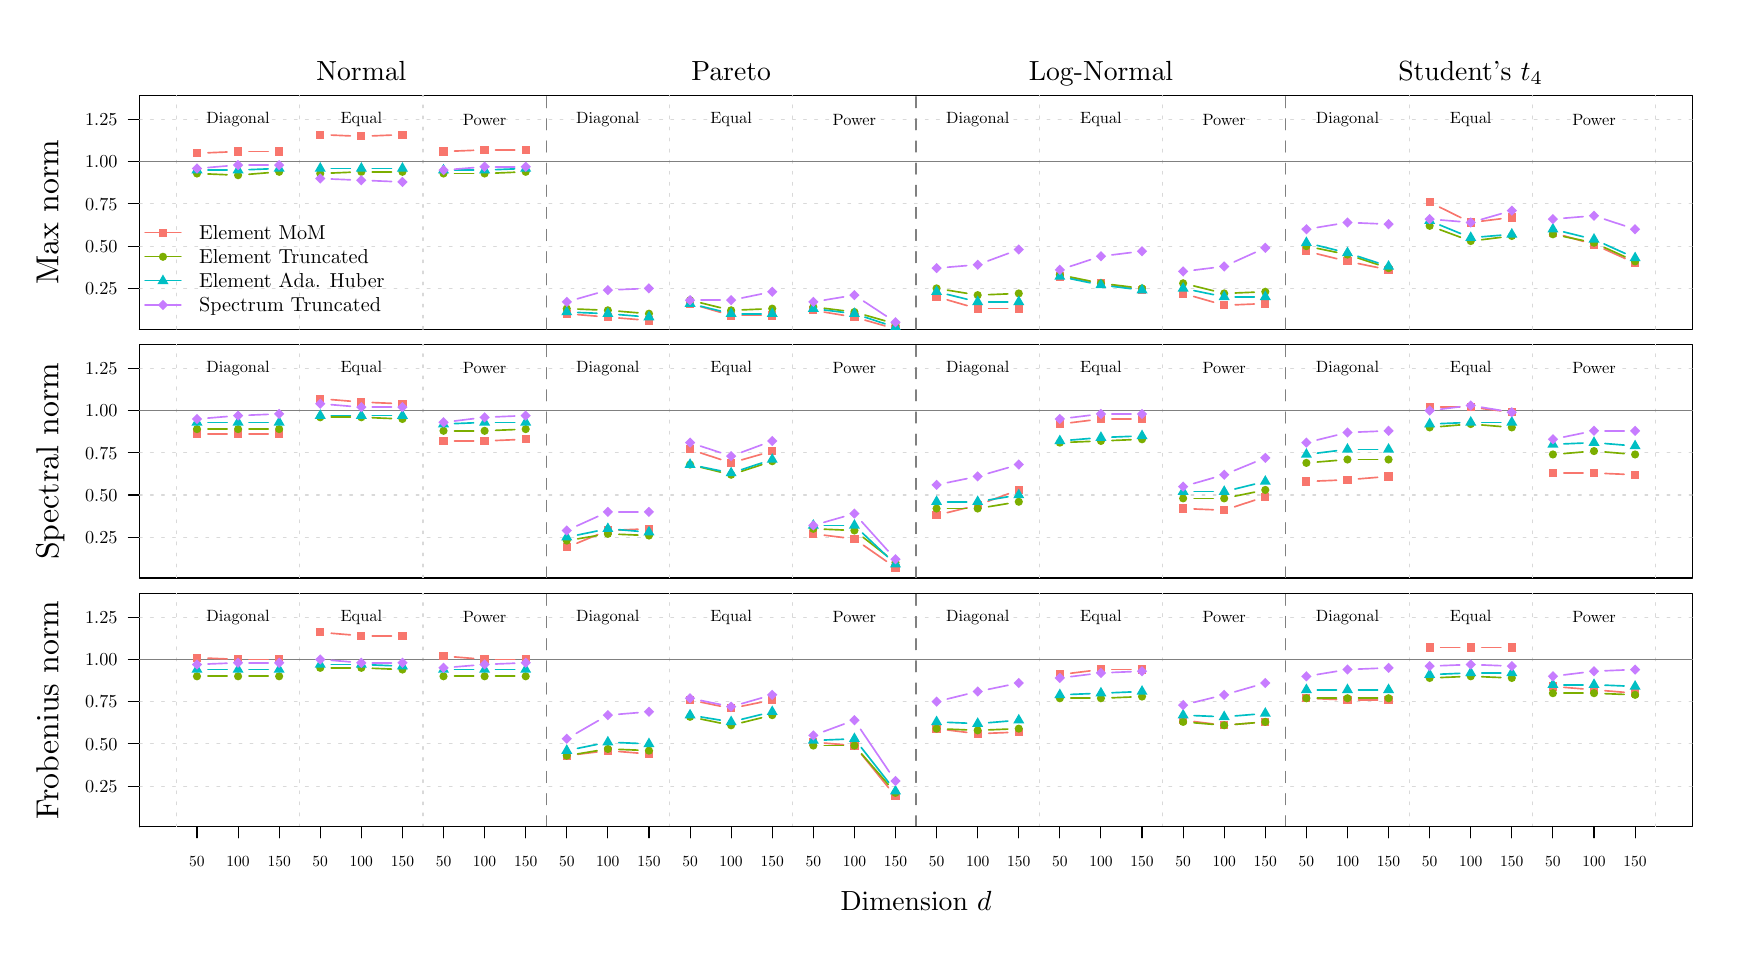
\begin{tikzpicture}[x=1pt,y=1pt]
\definecolor{fillColor}{RGB}{255,255,255}
\path[use as bounding box,fill=fillColor,fill opacity=0.00] (0,0) rectangle (614.29,325.21);
\begin{scope}
\path[clip] (  0.00,  0.00) rectangle (614.29,325.21);
\definecolor{drawColor}{RGB}{0,0,0}

\path[draw=drawColor,line width= 0.4pt,line join=round,line cap=round] ( 40.39,216.28) --
	(601.62,216.28) --
	(601.62,300.66) --
	( 40.39,300.66) --
	( 40.39,216.28);

\path[draw=drawColor,line width= 0.4pt,line join=round,line cap=round] ( 40.39,231.00) -- ( 40.39,292.04);

\path[draw=drawColor,line width= 0.4pt,line join=round,line cap=round] ( 40.39,231.00) -- ( 36.43,231.00);

\path[draw=drawColor,line width= 0.4pt,line join=round,line cap=round] ( 40.39,246.26) -- ( 36.43,246.26);

\path[draw=drawColor,line width= 0.4pt,line join=round,line cap=round] ( 40.39,261.52) -- ( 36.43,261.52);

\path[draw=drawColor,line width= 0.4pt,line join=round,line cap=round] ( 40.39,276.78) -- ( 36.43,276.78);

\path[draw=drawColor,line width= 0.4pt,line join=round,line cap=round] ( 40.39,292.04) -- ( 36.43,292.04);

\node[text=drawColor,anchor=base east,inner sep=0pt, outer sep=0pt, scale=  0.66] at ( 32.47,228.73) {0.25};

\node[text=drawColor,anchor=base east,inner sep=0pt, outer sep=0pt, scale=  0.66] at ( 32.47,243.99) {0.50};

\node[text=drawColor,anchor=base east,inner sep=0pt, outer sep=0pt, scale=  0.66] at ( 32.47,259.25) {0.75};

\node[text=drawColor,anchor=base east,inner sep=0pt, outer sep=0pt, scale=  0.66] at ( 32.47,274.51) {1.00};

\node[text=drawColor,anchor=base east,inner sep=0pt, outer sep=0pt, scale=  0.66] at ( 32.47,289.77) {1.25};
\end{scope}
\begin{scope}
\path[clip] ( 40.39,216.28) rectangle (601.62,300.66);
\definecolor{drawColor}{gray}{0.85}

\path[draw=drawColor,line width= 0.4pt,dash pattern=on 1pt off 3pt ,line join=round,line cap=round] ( 40.39,231.00) -- (601.62,231.00);

\path[draw=drawColor,line width= 0.4pt,dash pattern=on 1pt off 3pt ,line join=round,line cap=round] ( 40.39,246.26) -- (601.62,246.26);

\path[draw=drawColor,line width= 0.4pt,dash pattern=on 1pt off 3pt ,line join=round,line cap=round] ( 40.39,261.52) -- (601.62,261.52);

\path[draw=drawColor,line width= 0.4pt,dash pattern=on 1pt off 3pt ,line join=round,line cap=round] ( 40.39,276.78) -- (601.62,276.78);

\path[draw=drawColor,line width= 0.4pt,dash pattern=on 1pt off 3pt ,line join=round,line cap=round] ( 40.39,292.04) -- (601.62,292.04);

\path[draw=drawColor,line width= 0.4pt,dash pattern=on 1pt off 3pt ,line join=round,line cap=round] ( 98.30,216.28) -- ( 98.30,300.66);

\path[draw=drawColor,line width= 0.4pt,dash pattern=on 1pt off 3pt ,line join=round,line cap=round] (231.92,216.28) -- (231.92,300.66);

\path[draw=drawColor,line width= 0.4pt,dash pattern=on 1pt off 3pt ,line join=round,line cap=round] (365.55,216.28) -- (365.55,300.66);

\path[draw=drawColor,line width= 0.4pt,dash pattern=on 1pt off 3pt ,line join=round,line cap=round] (499.18,216.28) -- (499.18,300.66);

\path[draw=drawColor,line width= 0.4pt,dash pattern=on 1pt off 3pt ,line join=round,line cap=round] (142.84,216.28) -- (142.84,300.66);

\path[draw=drawColor,line width= 0.4pt,dash pattern=on 1pt off 3pt ,line join=round,line cap=round] (276.47,216.28) -- (276.47,300.66);

\path[draw=drawColor,line width= 0.4pt,dash pattern=on 1pt off 3pt ,line join=round,line cap=round] (410.09,216.28) -- (410.09,300.66);

\path[draw=drawColor,line width= 0.4pt,dash pattern=on 1pt off 3pt ,line join=round,line cap=round] (543.72,216.28) -- (543.72,300.66);

\path[draw=drawColor,line width= 0.4pt,dash pattern=on 1pt off 3pt ,line join=round,line cap=round] ( 53.75,216.28) -- ( 53.75,300.66);

\path[draw=drawColor,line width= 0.4pt,dash pattern=on 1pt off 3pt ,line join=round,line cap=round] (588.26,216.28) -- (588.26,300.66);
\definecolor{drawColor}{gray}{0.50}

\path[draw=drawColor,line width= 0.4pt,dash pattern=on 4pt off 4pt ,line join=round,line cap=round] (187.38,216.28) -- (187.38,300.66);

\path[draw=drawColor,line width= 0.4pt,dash pattern=on 4pt off 4pt ,line join=round,line cap=round] (321.01,216.28) -- (321.01,300.66);

\path[draw=drawColor,line width= 0.4pt,dash pattern=on 4pt off 4pt ,line join=round,line cap=round] (454.63,216.28) -- (454.63,300.66);
\end{scope}
\begin{scope}
\path[clip] (  0.00,  0.00) rectangle (614.29,325.21);
\definecolor{drawColor}{RGB}{0,0,0}

\node[text=drawColor,rotate= 90.00,anchor=base,inner sep=0pt, outer sep=0pt, scale=  1.15] at ( 11.09,258.47) {Max norm};
\end{scope}
\begin{scope}
\path[clip] ( 40.39,216.28) rectangle (601.62,300.66);
\definecolor{drawColor}{gray}{0.50}

\path[draw=drawColor,line width= 0.4pt,line join=round,line cap=round] ( 40.39,276.78) -- (601.62,276.78);
\end{scope}
\begin{scope}
\path[clip] (  0.00,  0.00) rectangle (614.29,325.21);
\definecolor{drawColor}{RGB}{0,0,0}

\node[text=drawColor,anchor=base,inner sep=0pt, outer sep=0pt, scale=  1.00] at (120.57,306.21) {Normal};

\node[text=drawColor,anchor=base,inner sep=0pt, outer sep=0pt, scale=  1.00] at (254.19,306.21) {Pareto};

\node[text=drawColor,anchor=base,inner sep=0pt, outer sep=0pt, scale=  1.00] at (387.82,306.21) {Log-Normal};

\node[text=drawColor,anchor=base,inner sep=0pt, outer sep=0pt, scale=  1.00] at (521.45,306.21) {Student's $t_4$};
\end{scope}
\begin{scope}
\path[clip] ( 40.39,216.28) rectangle (601.62,300.66);
\definecolor{drawColor}{RGB}{0,0,0}

\node[text=drawColor,anchor=base,inner sep=0pt, outer sep=0pt, scale=  0.59] at ( 76.03,290.58) {Diagonal};

\node[text=drawColor,anchor=base,inner sep=0pt, outer sep=0pt, scale=  0.59] at (120.57,290.58) {Equal};

\node[text=drawColor,anchor=base,inner sep=0pt, outer sep=0pt, scale=  0.59] at (165.11,290.00) {Power};

\node[text=drawColor,anchor=base,inner sep=0pt, outer sep=0pt, scale=  0.59] at (209.65,290.58) {Diagonal};

\node[text=drawColor,anchor=base,inner sep=0pt, outer sep=0pt, scale=  0.59] at (254.19,290.58) {Equal};

\node[text=drawColor,anchor=base,inner sep=0pt, outer sep=0pt, scale=  0.59] at (298.74,290.00) {Power};

\node[text=drawColor,anchor=base,inner sep=0pt, outer sep=0pt, scale=  0.59] at (343.28,290.58) {Diagonal};

\node[text=drawColor,anchor=base,inner sep=0pt, outer sep=0pt, scale=  0.59] at (387.82,290.58) {Equal};

\node[text=drawColor,anchor=base,inner sep=0pt, outer sep=0pt, scale=  0.59] at (432.36,290.00) {Power};

\node[text=drawColor,anchor=base,inner sep=0pt, outer sep=0pt, scale=  0.59] at (476.90,290.58) {Diagonal};

\node[text=drawColor,anchor=base,inner sep=0pt, outer sep=0pt, scale=  0.59] at (521.45,290.58) {Equal};

\node[text=drawColor,anchor=base,inner sep=0pt, outer sep=0pt, scale=  0.59] at (565.99,290.00) {Power};
\definecolor{drawColor}{RGB}{248,118,109}

\path[draw=drawColor,line width= 0.4pt,line join=round,line cap=round] ( 42.35,251.13) -- ( 55.42,251.13);
\definecolor{drawColor}{RGB}{124,174,0}

\path[draw=drawColor,line width= 0.4pt,line join=round,line cap=round] ( 42.35,242.42) -- ( 55.42,242.42);
\definecolor{drawColor}{RGB}{0,191,196}

\path[draw=drawColor,line width= 0.4pt,line join=round,line cap=round] ( 42.35,233.71) -- ( 55.42,233.71);
\definecolor{drawColor}{RGB}{199,124,255}

\path[draw=drawColor,line width= 0.4pt,line join=round,line cap=round] ( 42.35,224.99) -- ( 55.42,224.99);
\definecolor{fillColor}{RGB}{248,118,109}

\path[fill=fillColor] ( 47.40,249.64) --
	( 50.37,249.64) --
	( 50.37,252.61) --
	( 47.40,252.61) --
	cycle;
\definecolor{fillColor}{RGB}{124,174,0}

\path[fill=fillColor] ( 48.89,242.42) circle (  1.48);
\definecolor{fillColor}{RGB}{0,191,196}

\path[fill=fillColor] ( 48.89,236.02) --
	( 50.89,232.55) --
	( 46.89,232.55) --
	cycle;
\definecolor{fillColor}{RGB}{199,124,255}

\path[fill=fillColor] ( 47.03,224.99) --
	( 48.89,226.85) --
	( 50.74,224.99) --
	( 48.89,223.14) --
	cycle;
\definecolor{drawColor}{RGB}{0,0,0}

\node[text=drawColor,anchor=base west,inner sep=0pt, outer sep=0pt, scale=  0.73] at ( 61.95,248.63) {Element MoM};

\node[text=drawColor,anchor=base west,inner sep=0pt, outer sep=0pt, scale=  0.73] at ( 61.95,239.92) {Element Truncated};

\node[text=drawColor,anchor=base west,inner sep=0pt, outer sep=0pt, scale=  0.73] at ( 61.95,231.21) {Element Ada. Huber};

\node[text=drawColor,anchor=base west,inner sep=0pt, outer sep=0pt, scale=  0.73] at ( 61.95,222.49) {Spectrum Truncated};
\definecolor{drawColor}{RGB}{248,118,109}

\path[draw=drawColor,line width= 0.6pt,line join=round,line cap=round] ( 65.13,280.00) -- ( 72.07,280.28);

\path[draw=drawColor,line width= 0.6pt,line join=round,line cap=round] ( 79.99,280.45) -- ( 86.91,280.45);
\definecolor{fillColor}{RGB}{248,118,109}

\path[fill=fillColor] ( 59.69,278.35) --
	( 62.66,278.35) --
	( 62.66,281.32) --
	( 59.69,281.32) --
	cycle;

\path[fill=fillColor] ( 74.54,278.96) --
	( 77.51,278.96) --
	( 77.51,281.93) --
	( 74.54,281.93) --
	cycle;

\path[fill=fillColor] ( 89.39,278.96) --
	( 92.36,278.96) --
	( 92.36,281.93) --
	( 89.39,281.93) --
	cycle;
\definecolor{drawColor}{RGB}{124,174,0}

\path[draw=drawColor,line width= 0.6pt,line join=round,line cap=round] ( 65.13,272.35) -- ( 72.07,272.06);

\path[draw=drawColor,line width= 0.6pt,line join=round,line cap=round] ( 79.97,272.23) -- ( 86.93,272.80);
\definecolor{fillColor}{RGB}{124,174,0}

\path[fill=fillColor] ( 61.18,272.51) circle (  1.48);

\path[fill=fillColor] ( 76.03,271.90) circle (  1.48);

\path[fill=fillColor] ( 90.87,273.12) circle (  1.48);
\definecolor{drawColor}{RGB}{0,191,196}

\path[draw=drawColor,line width= 0.6pt,line join=round,line cap=round] ( 65.14,273.73) -- ( 72.07,273.73);

\path[draw=drawColor,line width= 0.6pt,line join=round,line cap=round] ( 79.98,273.90) -- ( 86.92,274.18);
\definecolor{fillColor}{RGB}{0,191,196}

\path[fill=fillColor] ( 61.18,276.04) --
	( 63.18,272.58) --
	( 59.18,272.58) --
	cycle;

\path[fill=fillColor] ( 76.03,276.04) --
	( 78.03,272.58) --
	( 74.03,272.58) --
	cycle;

\path[fill=fillColor] ( 90.87,276.65) --
	( 92.87,273.19) --
	( 88.87,273.19) --
	cycle;
\definecolor{drawColor}{RGB}{199,124,255}

\path[draw=drawColor,line width= 0.6pt,line join=round,line cap=round] ( 65.13,274.67) -- ( 72.08,275.24);

\path[draw=drawColor,line width= 0.6pt,line join=round,line cap=round] ( 79.99,275.56) -- ( 86.91,275.56);
\definecolor{fillColor}{RGB}{199,124,255}

\path[fill=fillColor] ( 59.32,274.34) --
	( 61.18,276.20) --
	( 63.03,274.34) --
	( 61.18,272.49) --
	cycle;

\path[fill=fillColor] ( 74.17,275.56) --
	( 76.03,277.42) --
	( 77.88,275.56) --
	( 76.03,273.71) --
	cycle;

\path[fill=fillColor] ( 89.02,275.56) --
	( 90.87,277.42) --
	( 92.73,275.56) --
	( 90.87,273.71) --
	cycle;
\definecolor{drawColor}{RGB}{248,118,109}

\path[draw=drawColor,line width= 0.6pt,line join=round,line cap=round] (109.68,286.39) -- (116.61,286.10);

\path[draw=drawColor,line width= 0.6pt,line join=round,line cap=round] (124.52,286.10) -- (131.46,286.39);
\definecolor{fillColor}{RGB}{248,118,109}

\path[fill=fillColor] (104.24,285.07) --
	(107.21,285.07) --
	(107.21,288.04) --
	(104.24,288.04) --
	cycle;

\path[fill=fillColor] (119.08,284.46) --
	(122.05,284.46) --
	(122.05,287.43) --
	(119.08,287.43) --
	cycle;

\path[fill=fillColor] (133.93,285.07) --
	(136.90,285.07) --
	(136.90,288.04) --
	(133.93,288.04) --
	cycle;
\definecolor{drawColor}{RGB}{124,174,0}

\path[draw=drawColor,line width= 0.6pt,line join=round,line cap=round] (109.68,272.67) -- (116.61,272.96);

\path[draw=drawColor,line width= 0.6pt,line join=round,line cap=round] (124.53,273.12) -- (131.46,273.12);
\definecolor{fillColor}{RGB}{124,174,0}

\path[fill=fillColor] (105.72,272.51) circle (  1.48);

\path[fill=fillColor] (120.57,273.12) circle (  1.48);

\path[fill=fillColor] (135.42,273.12) circle (  1.48);
\definecolor{drawColor}{RGB}{0,191,196}

\path[draw=drawColor,line width= 0.6pt,line join=round,line cap=round] (109.68,274.34) -- (116.61,274.34);

\path[draw=drawColor,line width= 0.6pt,line join=round,line cap=round] (124.53,274.34) -- (131.46,274.34);
\definecolor{fillColor}{RGB}{0,191,196}

\path[fill=fillColor] (105.72,276.65) --
	(107.72,273.19) --
	(103.72,273.19) --
	cycle;

\path[fill=fillColor] (120.57,276.65) --
	(122.57,273.19) --
	(118.57,273.19) --
	cycle;

\path[fill=fillColor] (135.42,276.65) --
	(137.42,273.19) --
	(133.42,273.19) --
	cycle;
\definecolor{drawColor}{RGB}{199,124,255}

\path[draw=drawColor,line width= 0.6pt,line join=round,line cap=round] (109.68,270.52) -- (116.61,270.23);

\path[draw=drawColor,line width= 0.6pt,line join=round,line cap=round] (124.52,269.91) -- (131.46,269.62);
\definecolor{fillColor}{RGB}{199,124,255}

\path[fill=fillColor] (103.86,270.68) --
	(105.72,272.54) --
	(107.58,270.68) --
	(105.72,268.82) --
	cycle;

\path[fill=fillColor] (118.71,270.07) --
	(120.57,271.93) --
	(122.42,270.07) --
	(120.57,268.21) --
	cycle;

\path[fill=fillColor] (133.56,269.46) --
	(135.42,271.32) --
	(137.27,269.46) --
	(135.42,267.60) --
	cycle;
\definecolor{drawColor}{RGB}{248,118,109}

\path[draw=drawColor,line width= 0.6pt,line join=round,line cap=round] (154.22,280.61) -- (161.15,280.89);

\path[draw=drawColor,line width= 0.6pt,line join=round,line cap=round] (169.07,281.06) -- (176.00,281.06);
\definecolor{fillColor}{RGB}{248,118,109}

\path[fill=fillColor] (148.78,278.96) --
	(151.75,278.96) --
	(151.75,281.93) --
	(148.78,281.93) --
	cycle;

\path[fill=fillColor] (163.62,279.57) --
	(166.60,279.57) --
	(166.60,282.54) --
	(163.62,282.54) --
	cycle;

\path[fill=fillColor] (178.47,279.57) --
	(181.44,279.57) --
	(181.44,282.54) --
	(178.47,282.54) --
	cycle;
\definecolor{drawColor}{RGB}{124,174,0}

\path[draw=drawColor,line width= 0.6pt,line join=round,line cap=round] (154.22,272.51) -- (161.15,272.51);

\path[draw=drawColor,line width= 0.6pt,line join=round,line cap=round] (169.07,272.67) -- (176.00,272.96);
\definecolor{fillColor}{RGB}{124,174,0}

\path[fill=fillColor] (150.26,272.51) circle (  1.48);

\path[fill=fillColor] (165.11,272.51) circle (  1.48);

\path[fill=fillColor] (179.96,273.12) circle (  1.48);
\definecolor{drawColor}{RGB}{0,191,196}

\path[draw=drawColor,line width= 0.6pt,line join=round,line cap=round] (154.22,273.73) -- (161.15,273.73);

\path[draw=drawColor,line width= 0.6pt,line join=round,line cap=round] (169.07,273.90) -- (176.00,274.18);
\definecolor{fillColor}{RGB}{0,191,196}

\path[fill=fillColor] (150.26,276.04) --
	(152.26,272.58) --
	(148.26,272.58) --
	cycle;

\path[fill=fillColor] (165.11,276.04) --
	(167.11,272.58) --
	(163.11,272.58) --
	cycle;

\path[fill=fillColor] (179.96,276.65) --
	(181.96,273.19) --
	(177.96,273.19) --
	cycle;
\definecolor{drawColor}{RGB}{199,124,255}

\path[draw=drawColor,line width= 0.6pt,line join=round,line cap=round] (154.21,274.06) -- (161.16,274.63);

\path[draw=drawColor,line width= 0.6pt,line join=round,line cap=round] (169.07,274.95) -- (176.00,274.95);
\definecolor{fillColor}{RGB}{199,124,255}

\path[fill=fillColor] (148.41,273.73) --
	(150.26,275.59) --
	(152.12,273.73) --
	(150.26,271.88) --
	cycle;

\path[fill=fillColor] (163.25,274.95) --
	(165.11,276.81) --
	(166.97,274.95) --
	(165.11,273.10) --
	cycle;

\path[fill=fillColor] (178.10,274.95) --
	(179.96,276.81) --
	(181.81,274.95) --
	(179.96,273.10) --
	cycle;
\definecolor{drawColor}{RGB}{248,118,109}

\path[draw=drawColor,line width= 0.6pt,line join=round,line cap=round] (198.75,221.52) -- (205.71,220.95);

\path[draw=drawColor,line width= 0.6pt,line join=round,line cap=round] (213.60,220.30) -- (220.55,219.73);
\definecolor{fillColor}{RGB}{248,118,109}

\path[fill=fillColor] (193.32,220.36) --
	(196.29,220.36) --
	(196.29,223.33) --
	(193.32,223.33) --
	cycle;

\path[fill=fillColor] (208.17,219.14) --
	(211.14,219.14) --
	(211.14,222.11) --
	(208.17,222.11) --
	cycle;

\path[fill=fillColor] (223.01,217.92) --
	(225.98,217.92) --
	(225.98,220.89) --
	(223.01,220.89) --
	cycle;
\definecolor{drawColor}{RGB}{124,174,0}

\path[draw=drawColor,line width= 0.6pt,line join=round,line cap=round] (198.76,223.52) -- (205.70,223.23);

\path[draw=drawColor,line width= 0.6pt,line join=round,line cap=round] (213.60,222.75) -- (220.55,222.17);
\definecolor{fillColor}{RGB}{124,174,0}

\path[fill=fillColor] (194.80,223.68) circle (  1.48);

\path[fill=fillColor] (209.65,223.07) circle (  1.48);

\path[fill=fillColor] (224.50,221.85) circle (  1.48);
\definecolor{drawColor}{RGB}{0,191,196}

\path[draw=drawColor,line width= 0.6pt,line join=round,line cap=round] (198.76,222.30) -- (205.70,222.01);

\path[draw=drawColor,line width= 0.6pt,line join=round,line cap=round] (213.60,221.52) -- (220.55,220.95);
\definecolor{fillColor}{RGB}{0,191,196}

\path[fill=fillColor] (194.80,224.77) --
	(196.80,221.30) --
	(192.80,221.30) --
	cycle;

\path[fill=fillColor] (209.65,224.16) --
	(211.65,220.69) --
	(207.65,220.69) --
	cycle;

\path[fill=fillColor] (224.50,222.94) --
	(226.50,219.47) --
	(222.50,219.47) --
	cycle;
\definecolor{drawColor}{RGB}{199,124,255}

\path[draw=drawColor,line width= 0.6pt,line join=round,line cap=round] (198.61,227.22) -- (205.85,229.30);

\path[draw=drawColor,line width= 0.6pt,line join=round,line cap=round] (213.61,230.56) -- (220.54,230.84);
\definecolor{fillColor}{RGB}{199,124,255}

\path[fill=fillColor] (192.95,226.12) --
	(194.80,227.98) --
	(196.66,226.12) --
	(194.80,224.27) --
	cycle;

\path[fill=fillColor] (207.80,230.39) --
	(209.65,232.25) --
	(211.51,230.39) --
	(209.65,228.54) --
	cycle;

\path[fill=fillColor] (222.64,231.00) --
	(224.50,232.86) --
	(226.36,231.00) --
	(224.50,229.15) --
	cycle;
\definecolor{drawColor}{RGB}{248,118,109}

\path[draw=drawColor,line width= 0.6pt,line join=round,line cap=round] (243.15,224.42) -- (250.39,222.33);

\path[draw=drawColor,line width= 0.6pt,line join=round,line cap=round] (258.15,221.24) -- (265.08,221.24);
\definecolor{fillColor}{RGB}{248,118,109}

\path[fill=fillColor] (237.86,224.03) --
	(240.83,224.03) --
	(240.83,227.00) --
	(237.86,227.00) --
	cycle;

\path[fill=fillColor] (252.71,219.75) --
	(255.68,219.75) --
	(255.68,222.72) --
	(252.71,222.72) --
	cycle;

\path[fill=fillColor] (267.56,219.75) --
	(270.53,219.75) --
	(270.53,222.72) --
	(267.56,222.72) --
	cycle;
\definecolor{drawColor}{RGB}{124,174,0}

\path[draw=drawColor,line width= 0.6pt,line join=round,line cap=round] (243.19,225.78) -- (250.35,224.02);

\path[draw=drawColor,line width= 0.6pt,line join=round,line cap=round] (258.15,223.23) -- (265.09,223.52);
\definecolor{fillColor}{RGB}{124,174,0}

\path[fill=fillColor] (239.35,226.73) circle (  1.48);

\path[fill=fillColor] (254.19,223.07) circle (  1.48);

\path[fill=fillColor] (269.04,223.68) circle (  1.48);
\definecolor{drawColor}{RGB}{0,191,196}

\path[draw=drawColor,line width= 0.6pt,line join=round,line cap=round] (243.19,224.56) -- (250.35,222.80);

\path[draw=drawColor,line width= 0.6pt,line join=round,line cap=round] (258.15,221.85) -- (265.08,221.85);
\definecolor{fillColor}{RGB}{0,191,196}

\path[fill=fillColor] (239.35,227.82) --
	(241.35,224.36) --
	(237.35,224.36) --
	cycle;

\path[fill=fillColor] (254.19,224.16) --
	(256.19,220.69) --
	(252.19,220.69) --
	cycle;

\path[fill=fillColor] (269.04,224.16) --
	(271.04,220.69) --
	(267.04,220.69) --
	cycle;
\definecolor{drawColor}{RGB}{199,124,255}

\path[draw=drawColor,line width= 0.6pt,line join=round,line cap=round] (243.31,226.73) -- (250.23,226.73);

\path[draw=drawColor,line width= 0.6pt,line join=round,line cap=round] (258.07,227.53) -- (265.16,228.99);
\definecolor{fillColor}{RGB}{199,124,255}

\path[fill=fillColor] (237.49,226.73) --
	(239.35,228.59) --
	(241.20,226.73) --
	(239.35,224.88) --
	cycle;

\path[fill=fillColor] (252.34,226.73) --
	(254.19,228.59) --
	(256.05,226.73) --
	(254.19,224.88) --
	cycle;

\path[fill=fillColor] (267.19,229.78) --
	(269.04,231.64) --
	(270.90,229.78) --
	(269.04,227.93) --
	cycle;
\definecolor{drawColor}{RGB}{248,118,109}

\path[draw=drawColor,line width= 0.6pt,line join=round,line cap=round] (287.80,222.43) -- (294.83,221.27);

\path[draw=drawColor,line width= 0.6pt,line join=round,line cap=round] (302.54,219.53) -- (309.78,217.45);
\definecolor{fillColor}{RGB}{248,118,109}

\path[fill=fillColor] (282.40,221.58) --
	(285.37,221.58) --
	(285.37,224.55) --
	(282.40,224.55) --
	cycle;

\path[fill=fillColor] (297.25,219.14) --
	(300.22,219.14) --
	(300.22,222.11) --
	(297.25,222.11) --
	cycle;

\path[fill=fillColor] (312.10,214.87) --
	(315.07,214.87) --
	(315.07,217.84) --
	(312.10,217.84) --
	cycle;
\definecolor{drawColor}{RGB}{124,174,0}

\path[draw=drawColor,line width= 0.6pt,line join=round,line cap=round] (287.82,223.81) -- (294.81,222.94);

\path[draw=drawColor,line width= 0.6pt,line join=round,line cap=round] (302.54,221.36) -- (309.78,219.28);
\definecolor{fillColor}{RGB}{124,174,0}

\path[fill=fillColor] (283.89,224.29) circle (  1.48);

\path[fill=fillColor] (298.74,222.46) circle (  1.48);

\path[fill=fillColor] (313.58,218.19) circle (  1.48);
\definecolor{drawColor}{RGB}{0,191,196}

\path[draw=drawColor,line width= 0.6pt,line join=round,line cap=round] (287.82,223.20) -- (294.81,222.33);

\path[draw=drawColor,line width= 0.6pt,line join=round,line cap=round] (302.50,220.61) -- (309.82,218.20);
\definecolor{fillColor}{RGB}{0,191,196}

\path[fill=fillColor] (283.89,225.99) --
	(285.89,222.53) --
	(281.89,222.53) --
	cycle;

\path[fill=fillColor] (298.74,224.16) --
	(300.74,220.69) --
	(296.74,220.69) --
	cycle;

\path[fill=fillColor] (313.58,219.27) --
	(315.58,215.81) --
	(311.58,215.81) --
	cycle;
\definecolor{drawColor}{RGB}{199,124,255}

\path[draw=drawColor,line width= 0.6pt,line join=round,line cap=round] (287.80,226.76) -- (294.83,227.92);

\path[draw=drawColor,line width= 0.6pt,line join=round,line cap=round] (302.04,226.39) -- (310.28,220.97);
\definecolor{fillColor}{RGB}{199,124,255}

\path[fill=fillColor] (282.03,226.12) --
	(283.89,227.98) --
	(285.75,226.12) --
	(283.89,224.27) --
	cycle;

\path[fill=fillColor] (296.88,228.56) --
	(298.74,230.42) --
	(300.59,228.56) --
	(298.74,226.71) --
	cycle;

\path[fill=fillColor] (311.73,218.80) --
	(313.58,220.65) --
	(315.44,218.80) --
	(313.58,216.94) --
	cycle;
\definecolor{drawColor}{RGB}{248,118,109}

\path[draw=drawColor,line width= 0.6pt,line join=round,line cap=round] (332.24,226.86) -- (339.47,224.78);

\path[draw=drawColor,line width= 0.6pt,line join=round,line cap=round] (347.24,223.68) -- (354.17,223.68);
\definecolor{fillColor}{RGB}{248,118,109}

\path[fill=fillColor] (326.95,226.47) --
	(329.92,226.47) --
	(329.92,229.44) --
	(326.95,229.44) --
	cycle;

\path[fill=fillColor] (341.79,222.19) --
	(344.76,222.19) --
	(344.76,225.16) --
	(341.79,225.16) --
	cycle;

\path[fill=fillColor] (356.64,222.19) --
	(359.61,222.19) --
	(359.61,225.16) --
	(356.64,225.16) --
	cycle;
\definecolor{drawColor}{RGB}{124,174,0}

\path[draw=drawColor,line width= 0.6pt,line join=round,line cap=round] (332.34,230.36) -- (339.37,229.21);

\path[draw=drawColor,line width= 0.6pt,line join=round,line cap=round] (347.24,228.73) -- (354.17,229.01);
\definecolor{fillColor}{RGB}{124,174,0}

\path[fill=fillColor] (328.43,231.00) circle (  1.48);

\path[fill=fillColor] (343.28,228.56) circle (  1.48);

\path[fill=fillColor] (358.13,229.17) circle (  1.48);
\definecolor{drawColor}{RGB}{0,191,196}

\path[draw=drawColor,line width= 0.6pt,line join=round,line cap=round] (332.28,228.84) -- (339.43,227.07);

\path[draw=drawColor,line width= 0.6pt,line join=round,line cap=round] (347.24,226.12) -- (354.17,226.12);
\definecolor{fillColor}{RGB}{0,191,196}

\path[fill=fillColor] (328.43,232.09) --
	(330.43,228.63) --
	(326.43,228.63) --
	cycle;

\path[fill=fillColor] (343.28,228.43) --
	(345.28,224.97) --
	(341.28,224.97) --
	cycle;

\path[fill=fillColor] (358.13,228.43) --
	(360.13,224.97) --
	(356.13,224.97) --
	cycle;
\definecolor{drawColor}{RGB}{199,124,255}

\path[draw=drawColor,line width= 0.6pt,line join=round,line cap=round] (332.38,238.65) -- (339.33,239.23);

\path[draw=drawColor,line width= 0.6pt,line join=round,line cap=round] (346.99,240.92) -- (354.41,243.67);
\definecolor{fillColor}{RGB}{199,124,255}

\path[fill=fillColor] (326.57,238.33) --
	(328.43,240.19) --
	(330.29,238.33) --
	(328.43,236.47) --
	cycle;

\path[fill=fillColor] (341.42,239.55) --
	(343.28,241.41) --
	(345.13,239.55) --
	(343.28,237.69) --
	cycle;

\path[fill=fillColor] (356.27,245.04) --
	(358.13,246.90) --
	(359.98,245.04) --
	(358.13,243.19) --
	cycle;
\definecolor{drawColor}{RGB}{248,118,109}

\path[draw=drawColor,line width= 0.6pt,line join=round,line cap=round] (376.88,234.63) -- (383.91,233.48);

\path[draw=drawColor,line width= 0.6pt,line join=round,line cap=round] (391.73,232.19) -- (398.76,231.04);
\definecolor{fillColor}{RGB}{248,118,109}

\path[fill=fillColor] (371.49,233.79) --
	(374.46,233.79) --
	(374.46,236.76) --
	(371.49,236.76) --
	cycle;

\path[fill=fillColor] (386.34,231.35) --
	(389.31,231.35) --
	(389.31,234.32) --
	(386.34,234.32) --
	cycle;

\path[fill=fillColor] (401.18,228.91) --
	(404.15,228.91) --
	(404.15,231.88) --
	(401.18,231.88) --
	cycle;
\definecolor{drawColor}{RGB}{124,174,0}

\path[draw=drawColor,line width= 0.6pt,line join=round,line cap=round] (376.85,235.09) -- (383.94,233.63);

\path[draw=drawColor,line width= 0.6pt,line join=round,line cap=round] (391.75,232.35) -- (398.74,231.49);
\definecolor{fillColor}{RGB}{124,174,0}

\path[fill=fillColor] (372.97,235.89) circle (  1.48);

\path[fill=fillColor] (387.82,232.84) circle (  1.48);

\path[fill=fillColor] (402.67,231.00) circle (  1.48);
\definecolor{drawColor}{RGB}{0,191,196}

\path[draw=drawColor,line width= 0.6pt,line join=round,line cap=round] (376.85,234.48) -- (383.94,233.02);

\path[draw=drawColor,line width= 0.6pt,line join=round,line cap=round] (391.75,231.74) -- (398.74,230.88);
\definecolor{fillColor}{RGB}{0,191,196}

\path[fill=fillColor] (372.97,237.59) --
	(374.97,234.12) --
	(370.97,234.12) --
	cycle;

\path[fill=fillColor] (387.82,234.53) --
	(389.82,231.07) --
	(385.82,231.07) --
	cycle;

\path[fill=fillColor] (402.67,232.70) --
	(404.67,229.24) --
	(400.67,229.24) --
	cycle;
\definecolor{drawColor}{RGB}{199,124,255}

\path[draw=drawColor,line width= 0.6pt,line join=round,line cap=round] (376.74,238.96) -- (384.06,241.37);

\path[draw=drawColor,line width= 0.6pt,line join=round,line cap=round] (391.75,243.09) -- (398.74,243.95);
\definecolor{fillColor}{RGB}{199,124,255}

\path[fill=fillColor] (371.12,237.72) --
	(372.97,239.58) --
	(374.83,237.72) --
	(372.97,235.86) --
	cycle;

\path[fill=fillColor] (385.96,242.60) --
	(387.82,244.46) --
	(389.68,242.60) --
	(387.82,240.75) --
	cycle;

\path[fill=fillColor] (400.81,244.43) --
	(402.67,246.29) --
	(404.52,244.43) --
	(402.67,242.58) --
	cycle;
\definecolor{drawColor}{RGB}{248,118,109}

\path[draw=drawColor,line width= 0.6pt,line join=round,line cap=round] (421.32,228.08) -- (428.56,226.00);

\path[draw=drawColor,line width= 0.6pt,line join=round,line cap=round] (436.32,225.06) -- (443.25,225.35);
\definecolor{fillColor}{RGB}{248,118,109}

\path[fill=fillColor] (416.03,227.69) --
	(419.00,227.69) --
	(419.00,230.66) --
	(416.03,230.66) --
	cycle;

\path[fill=fillColor] (430.88,223.42) --
	(433.85,223.42) --
	(433.85,226.39) --
	(430.88,226.39) --
	cycle;

\path[fill=fillColor] (445.73,224.03) --
	(448.70,224.03) --
	(448.70,227.00) --
	(445.73,227.00) --
	cycle;
\definecolor{drawColor}{RGB}{124,174,0}

\path[draw=drawColor,line width= 0.6pt,line join=round,line cap=round] (421.36,231.89) -- (428.52,230.12);

\path[draw=drawColor,line width= 0.6pt,line join=round,line cap=round] (436.32,229.34) -- (443.25,229.62);
\definecolor{fillColor}{RGB}{124,174,0}

\path[fill=fillColor] (417.52,232.84) circle (  1.48);

\path[fill=fillColor] (432.36,229.17) circle (  1.48);

\path[fill=fillColor] (447.21,229.78) circle (  1.48);
\definecolor{drawColor}{RGB}{0,191,196}

\path[draw=drawColor,line width= 0.6pt,line join=round,line cap=round] (421.39,230.21) -- (428.48,228.75);

\path[draw=drawColor,line width= 0.6pt,line join=round,line cap=round] (436.32,227.95) -- (443.25,227.95);
\definecolor{fillColor}{RGB}{0,191,196}

\path[fill=fillColor] (417.52,233.31) --
	(419.52,229.85) --
	(415.52,229.85) --
	cycle;

\path[fill=fillColor] (432.36,230.26) --
	(434.36,226.80) --
	(430.36,226.80) --
	cycle;

\path[fill=fillColor] (447.21,230.26) --
	(449.21,226.80) --
	(445.21,226.80) --
	cycle;
\definecolor{drawColor}{RGB}{199,124,255}

\path[draw=drawColor,line width= 0.6pt,line join=round,line cap=round] (421.45,237.59) -- (428.43,238.46);

\path[draw=drawColor,line width= 0.6pt,line join=round,line cap=round] (435.97,240.57) -- (443.60,244.02);
\definecolor{fillColor}{RGB}{199,124,255}

\path[fill=fillColor] (415.66,237.11) --
	(417.52,238.96) --
	(419.37,237.11) --
	(417.52,235.25) --
	cycle;

\path[fill=fillColor] (430.51,238.94) --
	(432.36,240.80) --
	(434.22,238.94) --
	(432.36,237.08) --
	cycle;

\path[fill=fillColor] (445.35,245.65) --
	(447.21,247.51) --
	(449.07,245.65) --
	(447.21,243.80) --
	cycle;
\definecolor{drawColor}{RGB}{248,118,109}

\path[draw=drawColor,line width= 0.6pt,line join=round,line cap=round] (465.90,243.49) -- (473.06,241.72);

\path[draw=drawColor,line width= 0.6pt,line join=round,line cap=round] (480.78,239.97) -- (487.87,238.52);
\definecolor{fillColor}{RGB}{248,118,109}

\path[fill=fillColor] (460.57,242.95) --
	(463.54,242.95) --
	(463.54,245.92) --
	(460.57,245.92) --
	cycle;

\path[fill=fillColor] (475.42,239.29) --
	(478.39,239.29) --
	(478.39,242.26) --
	(475.42,242.26) --
	cycle;

\path[fill=fillColor] (490.27,236.23) --
	(493.24,236.23) --
	(493.24,239.20) --
	(490.27,239.20) --
	cycle;
\definecolor{drawColor}{RGB}{124,174,0}

\path[draw=drawColor,line width= 0.6pt,line join=round,line cap=round] (465.94,245.47) -- (473.03,244.01);

\path[draw=drawColor,line width= 0.6pt,line join=round,line cap=round] (480.67,241.98) -- (487.99,239.57);
\definecolor{fillColor}{RGB}{124,174,0}

\path[fill=fillColor] (462.06,246.26) circle (  1.48);

\path[fill=fillColor] (476.90,243.21) circle (  1.48);

\path[fill=fillColor] (491.75,238.33) circle (  1.48);
\definecolor{drawColor}{RGB}{0,191,196}

\path[draw=drawColor,line width= 0.6pt,line join=round,line cap=round] (465.90,246.54) -- (473.06,244.77);

\path[draw=drawColor,line width= 0.6pt,line join=round,line cap=round] (480.67,242.59) -- (487.99,240.18);
\definecolor{fillColor}{RGB}{0,191,196}

\path[fill=fillColor] (462.06,249.79) --
	(464.06,246.33) --
	(460.06,246.33) --
	cycle;

\path[fill=fillColor] (476.90,246.13) --
	(478.90,242.67) --
	(474.91,242.67) --
	cycle;

\path[fill=fillColor] (491.75,241.25) --
	(493.75,237.79) --
	(489.75,237.79) --
	cycle;
\definecolor{drawColor}{RGB}{199,124,255}

\path[draw=drawColor,line width= 0.6pt,line join=round,line cap=round] (465.97,253.01) -- (473.00,254.17);

\path[draw=drawColor,line width= 0.6pt,line join=round,line cap=round] (480.86,254.65) -- (487.80,254.36);
\definecolor{fillColor}{RGB}{199,124,255}

\path[fill=fillColor] (460.20,252.37) --
	(462.06,254.22) --
	(463.91,252.37) --
	(462.06,250.51) --
	cycle;

\path[fill=fillColor] (475.05,254.81) --
	(476.90,256.67) --
	(478.76,254.81) --
	(476.90,252.95) --
	cycle;

\path[fill=fillColor] (489.90,254.20) --
	(491.75,256.06) --
	(493.61,254.20) --
	(491.75,252.34) --
	cycle;
\definecolor{drawColor}{RGB}{248,118,109}

\path[draw=drawColor,line width= 0.6pt,line join=round,line cap=round] (510.15,260.38) -- (517.90,256.56);

\path[draw=drawColor,line width= 0.6pt,line join=round,line cap=round] (525.38,255.29) -- (532.36,256.16);
\definecolor{fillColor}{RGB}{248,118,109}

\path[fill=fillColor] (505.11,260.65) --
	(508.08,260.65) --
	(508.08,263.62) --
	(505.11,263.62) --
	cycle;

\path[fill=fillColor] (519.96,253.33) --
	(522.93,253.33) --
	(522.93,256.30) --
	(519.96,256.30) --
	cycle;

\path[fill=fillColor] (534.81,255.16) --
	(537.78,255.16) --
	(537.78,258.13) --
	(534.81,258.13) --
	cycle;
\definecolor{drawColor}{RGB}{124,174,0}

\path[draw=drawColor,line width= 0.6pt,line join=round,line cap=round] (510.31,252.22) -- (517.73,249.47);

\path[draw=drawColor,line width= 0.6pt,line join=round,line cap=round] (525.38,248.58) -- (532.36,249.44);
\definecolor{fillColor}{RGB}{124,174,0}

\path[fill=fillColor] (506.60,253.59) circle (  1.48);

\path[fill=fillColor] (521.45,248.10) circle (  1.48);

\path[fill=fillColor] (536.29,249.93) circle (  1.48);
\definecolor{drawColor}{RGB}{0,191,196}

\path[draw=drawColor,line width= 0.6pt,line join=round,line cap=round] (510.26,253.91) -- (517.78,250.82);

\path[draw=drawColor,line width= 0.6pt,line join=round,line cap=round] (525.39,249.64) -- (532.35,250.21);
\definecolor{fillColor}{RGB}{0,191,196}

\path[fill=fillColor] (506.60,257.73) --
	(508.60,254.27) --
	(504.60,254.27) --
	cycle;

\path[fill=fillColor] (521.45,251.63) --
	(523.45,248.16) --
	(519.45,248.16) --
	cycle;

\path[fill=fillColor] (536.29,252.85) --
	(538.29,249.38) --
	(534.29,249.38) --
	cycle;
\definecolor{drawColor}{RGB}{199,124,255}

\path[draw=drawColor,line width= 0.6pt,line join=round,line cap=round] (510.55,255.71) -- (517.50,255.13);

\path[draw=drawColor,line width= 0.6pt,line join=round,line cap=round] (525.25,255.91) -- (532.49,257.99);
\definecolor{fillColor}{RGB}{199,124,255}

\path[fill=fillColor] (504.74,256.03) --
	(506.60,257.89) --
	(508.46,256.03) --
	(506.60,254.17) --
	cycle;

\path[fill=fillColor] (519.59,254.81) --
	(521.45,256.67) --
	(523.30,254.81) --
	(521.45,252.95) --
	cycle;

\path[fill=fillColor] (534.44,259.08) --
	(536.29,260.94) --
	(538.15,259.08) --
	(536.29,257.23) --
	cycle;
\definecolor{drawColor}{RGB}{248,118,109}

\path[draw=drawColor,line width= 0.6pt,line join=round,line cap=round] (554.95,250.05) -- (562.18,247.97);

\path[draw=drawColor,line width= 0.6pt,line join=round,line cap=round] (569.60,245.24) -- (577.23,241.79);
\definecolor{fillColor}{RGB}{248,118,109}

\path[fill=fillColor] (549.66,249.66) --
	(552.63,249.66) --
	(552.63,252.63) --
	(549.66,252.63) --
	cycle;

\path[fill=fillColor] (564.50,245.39) --
	(567.47,245.39) --
	(567.47,248.36) --
	(564.50,248.36) --
	cycle;

\path[fill=fillColor] (579.35,238.68) --
	(582.32,238.68) --
	(582.32,241.65) --
	(579.35,241.65) --
	cycle;
\definecolor{drawColor}{RGB}{124,174,0}

\path[draw=drawColor,line width= 0.6pt,line join=round,line cap=round] (555.02,249.74) -- (562.11,248.28);

\path[draw=drawColor,line width= 0.6pt,line join=round,line cap=round] (569.60,245.85) -- (577.23,242.40);
\definecolor{fillColor}{RGB}{124,174,0}

\path[fill=fillColor] (551.14,250.54) circle (  1.48);

\path[fill=fillColor] (565.99,247.49) circle (  1.48);

\path[fill=fillColor] (580.84,240.77) circle (  1.48);
\definecolor{drawColor}{RGB}{0,191,196}

\path[draw=drawColor,line width= 0.6pt,line join=round,line cap=round] (554.99,251.42) -- (562.14,249.65);

\path[draw=drawColor,line width= 0.6pt,line join=round,line cap=round] (569.60,247.07) -- (577.23,243.62);
\definecolor{fillColor}{RGB}{0,191,196}

\path[fill=fillColor] (551.14,254.68) --
	(553.14,251.21) --
	(549.14,251.21) --
	cycle;

\path[fill=fillColor] (565.99,251.02) --
	(567.99,247.55) --
	(563.99,247.55) --
	cycle;

\path[fill=fillColor] (580.84,244.30) --
	(582.84,240.84) --
	(578.84,240.84) --
	cycle;
\definecolor{drawColor}{RGB}{199,124,255}

\path[draw=drawColor,line width= 0.6pt,line join=round,line cap=round] (555.09,256.36) -- (562.04,256.93);

\path[draw=drawColor,line width= 0.6pt,line join=round,line cap=round] (569.75,256.01) -- (577.07,253.61);
\definecolor{fillColor}{RGB}{199,124,255}

\path[fill=fillColor] (549.29,256.03) --
	(551.14,257.89) --
	(553.00,256.03) --
	(551.14,254.17) --
	cycle;

\path[fill=fillColor] (564.13,257.25) --
	(565.99,259.11) --
	(567.85,257.25) --
	(565.99,255.40) --
	cycle;

\path[fill=fillColor] (578.98,252.37) --
	(580.84,254.22) --
	(582.69,252.37) --
	(580.84,250.51) --
	cycle;
\end{scope}
\begin{scope}
\path[clip] (  0.00,  0.00) rectangle (614.29,325.21);
\definecolor{drawColor}{RGB}{0,0,0}

\path[draw=drawColor,line width= 0.4pt,line join=round,line cap=round] ( 40.39,126.36) --
	(601.62,126.36) --
	(601.62,210.74) --
	( 40.39,210.74) --
	( 40.39,126.36);

\path[draw=drawColor,line width= 0.4pt,line join=round,line cap=round] ( 40.39,141.08) -- ( 40.39,202.12);

\path[draw=drawColor,line width= 0.4pt,line join=round,line cap=round] ( 40.39,141.08) -- ( 36.43,141.08);

\path[draw=drawColor,line width= 0.4pt,line join=round,line cap=round] ( 40.39,156.34) -- ( 36.43,156.34);

\path[draw=drawColor,line width= 0.4pt,line join=round,line cap=round] ( 40.39,171.60) -- ( 36.43,171.60);

\path[draw=drawColor,line width= 0.4pt,line join=round,line cap=round] ( 40.39,186.86) -- ( 36.43,186.86);

\path[draw=drawColor,line width= 0.4pt,line join=round,line cap=round] ( 40.39,202.12) -- ( 36.43,202.12);

\node[text=drawColor,anchor=base east,inner sep=0pt, outer sep=0pt, scale=  0.66] at ( 32.47,138.81) {0.25};

\node[text=drawColor,anchor=base east,inner sep=0pt, outer sep=0pt, scale=  0.66] at ( 32.47,154.07) {0.50};

\node[text=drawColor,anchor=base east,inner sep=0pt, outer sep=0pt, scale=  0.66] at ( 32.47,169.33) {0.75};

\node[text=drawColor,anchor=base east,inner sep=0pt, outer sep=0pt, scale=  0.66] at ( 32.47,184.59) {1.00};

\node[text=drawColor,anchor=base east,inner sep=0pt, outer sep=0pt, scale=  0.66] at ( 32.47,199.85) {1.25};
\end{scope}
\begin{scope}
\path[clip] ( 40.39,126.36) rectangle (601.62,210.74);
\definecolor{drawColor}{gray}{0.85}

\path[draw=drawColor,line width= 0.4pt,dash pattern=on 1pt off 3pt ,line join=round,line cap=round] ( 40.39,141.08) -- (601.62,141.08);

\path[draw=drawColor,line width= 0.4pt,dash pattern=on 1pt off 3pt ,line join=round,line cap=round] ( 40.39,156.34) -- (601.62,156.34);

\path[draw=drawColor,line width= 0.4pt,dash pattern=on 1pt off 3pt ,line join=round,line cap=round] ( 40.39,171.60) -- (601.62,171.60);

\path[draw=drawColor,line width= 0.4pt,dash pattern=on 1pt off 3pt ,line join=round,line cap=round] ( 40.39,186.86) -- (601.62,186.86);

\path[draw=drawColor,line width= 0.4pt,dash pattern=on 1pt off 3pt ,line join=round,line cap=round] ( 40.39,202.12) -- (601.62,202.12);

\path[draw=drawColor,line width= 0.4pt,dash pattern=on 1pt off 3pt ,line join=round,line cap=round] ( 98.30,126.36) -- ( 98.30,210.74);

\path[draw=drawColor,line width= 0.4pt,dash pattern=on 1pt off 3pt ,line join=round,line cap=round] (231.92,126.36) -- (231.92,210.74);

\path[draw=drawColor,line width= 0.4pt,dash pattern=on 1pt off 3pt ,line join=round,line cap=round] (365.55,126.36) -- (365.55,210.74);

\path[draw=drawColor,line width= 0.4pt,dash pattern=on 1pt off 3pt ,line join=round,line cap=round] (499.18,126.36) -- (499.18,210.74);

\path[draw=drawColor,line width= 0.4pt,dash pattern=on 1pt off 3pt ,line join=round,line cap=round] (142.84,126.36) -- (142.84,210.74);

\path[draw=drawColor,line width= 0.4pt,dash pattern=on 1pt off 3pt ,line join=round,line cap=round] (276.47,126.36) -- (276.47,210.74);

\path[draw=drawColor,line width= 0.4pt,dash pattern=on 1pt off 3pt ,line join=round,line cap=round] (410.09,126.36) -- (410.09,210.74);

\path[draw=drawColor,line width= 0.4pt,dash pattern=on 1pt off 3pt ,line join=round,line cap=round] (543.72,126.36) -- (543.72,210.74);

\path[draw=drawColor,line width= 0.4pt,dash pattern=on 1pt off 3pt ,line join=round,line cap=round] ( 53.75,126.36) -- ( 53.75,210.74);

\path[draw=drawColor,line width= 0.4pt,dash pattern=on 1pt off 3pt ,line join=round,line cap=round] (588.26,126.36) -- (588.26,210.74);
\definecolor{drawColor}{gray}{0.50}

\path[draw=drawColor,line width= 0.4pt,dash pattern=on 4pt off 4pt ,line join=round,line cap=round] (187.38,126.36) -- (187.38,210.74);

\path[draw=drawColor,line width= 0.4pt,dash pattern=on 4pt off 4pt ,line join=round,line cap=round] (321.01,126.36) -- (321.01,210.74);

\path[draw=drawColor,line width= 0.4pt,dash pattern=on 4pt off 4pt ,line join=round,line cap=round] (454.63,126.36) -- (454.63,210.74);
\end{scope}
\begin{scope}
\path[clip] (  0.00,  0.00) rectangle (614.29,325.21);
\definecolor{drawColor}{RGB}{0,0,0}

\node[text=drawColor,rotate= 90.00,anchor=base,inner sep=0pt, outer sep=0pt, scale=  1.15] at ( 11.09,168.55) {Spectral norm};
\end{scope}
\begin{scope}
\path[clip] ( 40.39,126.36) rectangle (601.62,210.74);
\definecolor{drawColor}{gray}{0.50}

\path[draw=drawColor,line width= 0.4pt,line join=round,line cap=round] ( 40.39,186.86) -- (601.62,186.86);
\definecolor{drawColor}{RGB}{0,0,0}

\node[text=drawColor,anchor=base,inner sep=0pt, outer sep=0pt, scale=  0.59] at ( 76.03,200.65) {Diagonal};

\node[text=drawColor,anchor=base,inner sep=0pt, outer sep=0pt, scale=  0.59] at (120.57,200.65) {Equal};

\node[text=drawColor,anchor=base,inner sep=0pt, outer sep=0pt, scale=  0.59] at (165.11,200.07) {Power};

\node[text=drawColor,anchor=base,inner sep=0pt, outer sep=0pt, scale=  0.59] at (209.65,200.65) {Diagonal};

\node[text=drawColor,anchor=base,inner sep=0pt, outer sep=0pt, scale=  0.59] at (254.19,200.65) {Equal};

\node[text=drawColor,anchor=base,inner sep=0pt, outer sep=0pt, scale=  0.59] at (298.74,200.07) {Power};

\node[text=drawColor,anchor=base,inner sep=0pt, outer sep=0pt, scale=  0.59] at (343.28,200.65) {Diagonal};

\node[text=drawColor,anchor=base,inner sep=0pt, outer sep=0pt, scale=  0.59] at (387.82,200.65) {Equal};

\node[text=drawColor,anchor=base,inner sep=0pt, outer sep=0pt, scale=  0.59] at (432.36,200.07) {Power};

\node[text=drawColor,anchor=base,inner sep=0pt, outer sep=0pt, scale=  0.59] at (476.90,200.65) {Diagonal};

\node[text=drawColor,anchor=base,inner sep=0pt, outer sep=0pt, scale=  0.59] at (521.45,200.65) {Equal};

\node[text=drawColor,anchor=base,inner sep=0pt, outer sep=0pt, scale=  0.59] at (565.99,200.07) {Power};
\definecolor{drawColor}{RGB}{248,118,109}

\path[draw=drawColor,line width= 0.6pt,line join=round,line cap=round] ( 65.14,178.31) -- ( 72.07,178.31);

\path[draw=drawColor,line width= 0.6pt,line join=round,line cap=round] ( 79.99,178.31) -- ( 86.91,178.31);
\definecolor{fillColor}{RGB}{248,118,109}

\path[fill=fillColor] ( 59.69,176.83) --
	( 62.66,176.83) --
	( 62.66,179.80) --
	( 59.69,179.80) --
	cycle;

\path[fill=fillColor] ( 74.54,176.83) --
	( 77.51,176.83) --
	( 77.51,179.80) --
	( 74.54,179.80) --
	cycle;

\path[fill=fillColor] ( 89.39,176.83) --
	( 92.36,176.83) --
	( 92.36,179.80) --
	( 89.39,179.80) --
	cycle;
\definecolor{drawColor}{RGB}{124,174,0}

\path[draw=drawColor,line width= 0.6pt,line join=round,line cap=round] ( 65.14,180.15) -- ( 72.07,180.15);

\path[draw=drawColor,line width= 0.6pt,line join=round,line cap=round] ( 79.99,180.15) -- ( 86.91,180.15);
\definecolor{fillColor}{RGB}{124,174,0}

\path[fill=fillColor] ( 61.18,180.15) circle (  1.48);

\path[fill=fillColor] ( 76.03,180.15) circle (  1.48);

\path[fill=fillColor] ( 90.87,180.15) circle (  1.48);
\definecolor{drawColor}{RGB}{0,191,196}

\path[draw=drawColor,line width= 0.6pt,line join=round,line cap=round] ( 65.14,182.59) -- ( 72.07,182.59);

\path[draw=drawColor,line width= 0.6pt,line join=round,line cap=round] ( 79.99,182.59) -- ( 86.91,182.59);
\definecolor{fillColor}{RGB}{0,191,196}

\path[fill=fillColor] ( 61.18,184.90) --
	( 63.18,181.43) --
	( 59.18,181.43) --
	cycle;

\path[fill=fillColor] ( 76.03,184.90) --
	( 78.03,181.43) --
	( 74.03,181.43) --
	cycle;

\path[fill=fillColor] ( 90.87,184.90) --
	( 92.87,181.43) --
	( 88.87,181.43) --
	cycle;
\definecolor{drawColor}{RGB}{199,124,255}

\path[draw=drawColor,line width= 0.6pt,line join=round,line cap=round] ( 65.13,184.13) -- ( 72.08,184.70);

\path[draw=drawColor,line width= 0.6pt,line join=round,line cap=round] ( 79.98,185.19) -- ( 86.92,185.48);
\definecolor{fillColor}{RGB}{199,124,255}

\path[fill=fillColor] ( 59.32,183.81) --
	( 61.18,185.66) --
	( 63.03,183.81) --
	( 61.18,181.95) --
	cycle;

\path[fill=fillColor] ( 74.17,185.03) --
	( 76.03,186.88) --
	( 77.88,185.03) --
	( 76.03,183.17) --
	cycle;

\path[fill=fillColor] ( 89.02,185.64) --
	( 90.87,187.49) --
	( 92.73,185.64) --
	( 90.87,183.78) --
	cycle;
\definecolor{drawColor}{RGB}{248,118,109}

\path[draw=drawColor,line width= 0.6pt,line join=round,line cap=round] (109.67,190.81) -- (116.62,190.24);

\path[draw=drawColor,line width= 0.6pt,line join=round,line cap=round] (124.52,189.75) -- (131.46,189.46);
\definecolor{fillColor}{RGB}{248,118,109}

\path[fill=fillColor] (104.24,189.65) --
	(107.21,189.65) --
	(107.21,192.62) --
	(104.24,192.62) --
	cycle;

\path[fill=fillColor] (119.08,188.43) --
	(122.05,188.43) --
	(122.05,191.40) --
	(119.08,191.40) --
	cycle;

\path[fill=fillColor] (133.93,187.82) --
	(136.90,187.82) --
	(136.90,190.79) --
	(133.93,190.79) --
	cycle;
\definecolor{drawColor}{RGB}{124,174,0}

\path[draw=drawColor,line width= 0.6pt,line join=round,line cap=round] (109.68,184.42) -- (116.61,184.42);

\path[draw=drawColor,line width= 0.6pt,line join=round,line cap=round] (124.52,184.26) -- (131.46,183.97);
\definecolor{fillColor}{RGB}{124,174,0}

\path[fill=fillColor] (105.72,184.42) circle (  1.48);

\path[fill=fillColor] (120.57,184.42) circle (  1.48);

\path[fill=fillColor] (135.42,183.81) circle (  1.48);
\definecolor{drawColor}{RGB}{0,191,196}

\path[draw=drawColor,line width= 0.6pt,line join=round,line cap=round] (109.68,185.03) -- (116.61,185.03);

\path[draw=drawColor,line width= 0.6pt,line join=round,line cap=round] (124.53,185.03) -- (131.46,185.03);
\definecolor{fillColor}{RGB}{0,191,196}

\path[fill=fillColor] (105.72,187.34) --
	(107.72,183.87) --
	(103.72,183.87) --
	cycle;

\path[fill=fillColor] (120.57,187.34) --
	(122.57,183.87) --
	(118.57,183.87) --
	cycle;

\path[fill=fillColor] (135.42,187.34) --
	(137.42,183.87) --
	(133.42,183.87) --
	cycle;
\definecolor{drawColor}{RGB}{199,124,255}

\path[draw=drawColor,line width= 0.6pt,line join=round,line cap=round] (109.67,188.98) -- (116.62,188.40);

\path[draw=drawColor,line width= 0.6pt,line join=round,line cap=round] (124.53,188.08) -- (131.46,188.08);
\definecolor{fillColor}{RGB}{199,124,255}

\path[fill=fillColor] (103.86,189.30) --
	(105.72,191.16) --
	(107.58,189.30) --
	(105.72,187.44) --
	cycle;

\path[fill=fillColor] (118.71,188.08) --
	(120.57,189.94) --
	(122.42,188.08) --
	(120.57,186.22) --
	cycle;

\path[fill=fillColor] (133.56,188.08) --
	(135.42,189.94) --
	(137.27,188.08) --
	(135.42,186.22) --
	cycle;
\definecolor{drawColor}{RGB}{248,118,109}

\path[draw=drawColor,line width= 0.6pt,line join=round,line cap=round] (154.22,175.87) -- (161.15,175.87);

\path[draw=drawColor,line width= 0.6pt,line join=round,line cap=round] (169.07,176.03) -- (176.00,176.32);
\definecolor{fillColor}{RGB}{248,118,109}

\path[fill=fillColor] (148.78,174.39) --
	(151.75,174.39) --
	(151.75,177.36) --
	(148.78,177.36) --
	cycle;

\path[fill=fillColor] (163.62,174.39) --
	(166.60,174.39) --
	(166.60,177.36) --
	(163.62,177.36) --
	cycle;

\path[fill=fillColor] (178.47,175.00) --
	(181.44,175.00) --
	(181.44,177.97) --
	(178.47,177.97) --
	cycle;
\definecolor{drawColor}{RGB}{124,174,0}

\path[draw=drawColor,line width= 0.6pt,line join=round,line cap=round] (154.22,179.53) -- (161.15,179.53);

\path[draw=drawColor,line width= 0.6pt,line join=round,line cap=round] (169.07,179.70) -- (176.00,179.98);
\definecolor{fillColor}{RGB}{124,174,0}

\path[fill=fillColor] (150.26,179.53) circle (  1.48);

\path[fill=fillColor] (165.11,179.53) circle (  1.48);

\path[fill=fillColor] (179.96,180.15) circle (  1.48);
\definecolor{drawColor}{RGB}{0,191,196}

\path[draw=drawColor,line width= 0.6pt,line join=round,line cap=round] (154.22,182.14) -- (161.15,182.42);

\path[draw=drawColor,line width= 0.6pt,line join=round,line cap=round] (169.07,182.59) -- (176.00,182.59);
\definecolor{fillColor}{RGB}{0,191,196}

\path[fill=fillColor] (150.26,184.29) --
	(152.26,180.82) --
	(148.26,180.82) --
	cycle;

\path[fill=fillColor] (165.11,184.90) --
	(167.11,181.43) --
	(163.11,181.43) --
	cycle;

\path[fill=fillColor] (179.96,184.90) --
	(181.96,181.43) --
	(177.96,181.43) --
	cycle;
\definecolor{drawColor}{RGB}{199,124,255}

\path[draw=drawColor,line width= 0.6pt,line join=round,line cap=round] (154.19,183.07) -- (161.18,183.93);

\path[draw=drawColor,line width= 0.6pt,line join=round,line cap=round] (169.07,184.58) -- (176.00,184.87);
\definecolor{fillColor}{RGB}{199,124,255}

\path[fill=fillColor] (148.41,182.59) --
	(150.26,184.44) --
	(152.12,182.59) --
	(150.26,180.73) --
	cycle;

\path[fill=fillColor] (163.25,184.42) --
	(165.11,186.27) --
	(166.97,184.42) --
	(165.11,182.56) --
	cycle;

\path[fill=fillColor] (178.10,185.03) --
	(179.96,186.88) --
	(181.81,185.03) --
	(179.96,183.17) --
	cycle;
\definecolor{drawColor}{RGB}{248,118,109}

\path[draw=drawColor,line width= 0.6pt,line join=round,line cap=round] (198.47,138.92) -- (205.99,142.02);

\path[draw=drawColor,line width= 0.6pt,line join=round,line cap=round] (213.61,143.68) -- (220.54,143.97);
\definecolor{fillColor}{RGB}{248,118,109}

\path[fill=fillColor] (193.32,135.93) --
	(196.29,135.93) --
	(196.29,138.90) --
	(193.32,138.90) --
	cycle;

\path[fill=fillColor] (208.17,142.04) --
	(211.14,142.04) --
	(211.14,145.01) --
	(208.17,145.01) --
	cycle;

\path[fill=fillColor] (223.01,142.65) --
	(225.98,142.65) --
	(225.98,145.62) --
	(223.01,145.62) --
	cycle;
\definecolor{drawColor}{RGB}{124,174,0}

\path[draw=drawColor,line width= 0.6pt,line join=round,line cap=round] (198.71,140.50) -- (205.74,141.66);

\path[draw=drawColor,line width= 0.6pt,line join=round,line cap=round] (213.61,142.14) -- (220.54,141.85);
\definecolor{fillColor}{RGB}{124,174,0}

\path[fill=fillColor] (194.80,139.86) circle (  1.48);

\path[fill=fillColor] (209.65,142.30) circle (  1.48);

\path[fill=fillColor] (224.50,141.69) circle (  1.48);
\definecolor{drawColor}{RGB}{0,191,196}

\path[draw=drawColor,line width= 0.6pt,line join=round,line cap=round] (198.68,141.88) -- (205.77,143.33);

\path[draw=drawColor,line width= 0.6pt,line join=round,line cap=round] (213.60,143.81) -- (220.55,143.24);
\definecolor{fillColor}{RGB}{0,191,196}

\path[fill=fillColor] (194.80,143.39) --
	(196.80,139.93) --
	(192.80,139.93) --
	cycle;

\path[fill=fillColor] (209.65,146.44) --
	(211.65,142.98) --
	(207.65,142.98) --
	cycle;

\path[fill=fillColor] (224.50,145.22) --
	(226.50,141.76) --
	(222.50,141.76) --
	cycle;
\definecolor{drawColor}{RGB}{199,124,255}

\path[draw=drawColor,line width= 0.6pt,line join=round,line cap=round] (198.41,145.15) -- (206.04,148.60);

\path[draw=drawColor,line width= 0.6pt,line join=round,line cap=round] (213.61,150.24) -- (220.54,150.24);
\definecolor{fillColor}{RGB}{199,124,255}

\path[fill=fillColor] (192.95,143.52) --
	(194.80,145.38) --
	(196.66,143.52) --
	(194.80,141.67) --
	cycle;

\path[fill=fillColor] (207.80,150.24) --
	(209.65,152.09) --
	(211.51,150.24) --
	(209.65,148.38) --
	cycle;

\path[fill=fillColor] (222.64,150.24) --
	(224.50,152.09) --
	(226.36,150.24) --
	(224.50,148.38) --
	cycle;
\definecolor{drawColor}{RGB}{248,118,109}

\path[draw=drawColor,line width= 0.6pt,line join=round,line cap=round] (243.11,171.58) -- (250.43,169.17);

\path[draw=drawColor,line width= 0.6pt,line join=round,line cap=round] (258.00,169.03) -- (265.24,171.11);
\definecolor{fillColor}{RGB}{248,118,109}

\path[fill=fillColor] (237.86,171.34) --
	(240.83,171.34) --
	(240.83,174.31) --
	(237.86,174.31) --
	cycle;

\path[fill=fillColor] (252.71,166.45) --
	(255.68,166.45) --
	(255.68,169.42) --
	(252.71,169.42) --
	cycle;

\path[fill=fillColor] (267.56,170.72) --
	(270.53,170.72) --
	(270.53,173.69) --
	(267.56,173.69) --
	cycle;
\definecolor{drawColor}{RGB}{124,174,0}

\path[draw=drawColor,line width= 0.6pt,line join=round,line cap=round] (243.19,166.38) -- (250.35,164.61);

\path[draw=drawColor,line width= 0.6pt,line join=round,line cap=round] (257.96,164.90) -- (265.28,167.31);
\definecolor{fillColor}{RGB}{124,174,0}

\path[fill=fillColor] (239.35,167.33) circle (  1.48);

\path[fill=fillColor] (254.19,163.66) circle (  1.48);

\path[fill=fillColor] (269.04,168.55) circle (  1.48);
\definecolor{drawColor}{RGB}{0,191,196}

\path[draw=drawColor,line width= 0.6pt,line join=round,line cap=round] (243.23,166.53) -- (250.32,165.07);

\path[draw=drawColor,line width= 0.6pt,line join=round,line cap=round] (257.96,165.51) -- (265.28,167.92);
\definecolor{fillColor}{RGB}{0,191,196}

\path[fill=fillColor] (239.35,169.64) --
	(241.35,166.17) --
	(237.35,166.17) --
	cycle;

\path[fill=fillColor] (254.19,166.58) --
	(256.19,163.12) --
	(252.19,163.12) --
	cycle;

\path[fill=fillColor] (269.04,171.47) --
	(271.04,168.00) --
	(267.04,168.00) --
	cycle;
\definecolor{drawColor}{RGB}{199,124,255}

\path[draw=drawColor,line width= 0.6pt,line join=round,line cap=round] (243.11,174.02) -- (250.43,171.62);

\path[draw=drawColor,line width= 0.6pt,line join=round,line cap=round] (257.91,171.75) -- (265.33,174.50);
\definecolor{fillColor}{RGB}{199,124,255}

\path[fill=fillColor] (237.49,175.26) --
	(239.35,177.12) --
	(241.20,175.26) --
	(239.35,173.41) --
	cycle;

\path[fill=fillColor] (252.34,170.38) --
	(254.19,172.23) --
	(256.05,170.38) --
	(254.19,168.52) --
	cycle;

\path[fill=fillColor] (267.19,175.87) --
	(269.04,177.73) --
	(270.90,175.87) --
	(269.04,174.02) --
	cycle;
\definecolor{drawColor}{RGB}{248,118,109}

\path[draw=drawColor,line width= 0.6pt,line join=round,line cap=round] (287.82,141.82) -- (294.81,140.95);

\path[draw=drawColor,line width= 0.6pt,line join=round,line cap=round] (301.98,138.20) -- (310.34,132.36);
\definecolor{fillColor}{RGB}{248,118,109}

\path[fill=fillColor] (282.40,140.82) --
	(285.37,140.82) --
	(285.37,143.79) --
	(282.40,143.79) --
	cycle;

\path[fill=fillColor] (297.25,138.98) --
	(300.22,138.98) --
	(300.22,141.95) --
	(297.25,141.95) --
	cycle;

\path[fill=fillColor] (312.10,128.61) --
	(315.07,128.61) --
	(315.07,131.58) --
	(312.10,131.58) --
	cycle;
\definecolor{drawColor}{RGB}{124,174,0}

\path[draw=drawColor,line width= 0.6pt,line join=round,line cap=round] (287.85,143.97) -- (294.78,143.68);

\path[draw=drawColor,line width= 0.6pt,line join=round,line cap=round] (301.86,141.08) -- (310.46,134.36);
\definecolor{fillColor}{RGB}{124,174,0}

\path[fill=fillColor] (283.89,144.13) circle (  1.48);

\path[fill=fillColor] (298.74,143.52) circle (  1.48);

\path[fill=fillColor] (313.58,131.92) circle (  1.48);
\definecolor{drawColor}{RGB}{0,191,196}

\path[draw=drawColor,line width= 0.6pt,line join=round,line cap=round] (287.85,145.35) -- (294.78,145.35);

\path[draw=drawColor,line width= 0.6pt,line join=round,line cap=round] (301.61,142.63) -- (310.71,134.03);
\definecolor{fillColor}{RGB}{0,191,196}

\path[fill=fillColor] (283.89,147.66) --
	(285.89,144.20) --
	(281.89,144.20) --
	cycle;

\path[fill=fillColor] (298.74,147.66) --
	(300.74,144.20) --
	(296.74,144.20) --
	cycle;

\path[fill=fillColor] (313.58,133.62) --
	(315.58,130.16) --
	(311.58,130.16) --
	cycle;
\definecolor{drawColor}{RGB}{199,124,255}

\path[draw=drawColor,line width= 0.6pt,line join=round,line cap=round] (287.69,146.45) -- (294.93,148.53);

\path[draw=drawColor,line width= 0.6pt,line join=round,line cap=round] (301.39,146.68) -- (310.93,136.09);
\definecolor{fillColor}{RGB}{199,124,255}

\path[fill=fillColor] (282.03,145.35) --
	(283.89,147.21) --
	(285.75,145.35) --
	(283.89,143.50) --
	cycle;

\path[fill=fillColor] (296.88,149.63) --
	(298.74,151.48) --
	(300.59,149.63) --
	(298.74,147.77) --
	cycle;

\path[fill=fillColor] (311.73,133.14) --
	(313.58,135.00) --
	(315.44,133.14) --
	(313.58,131.29) --
	cycle;
\definecolor{drawColor}{RGB}{248,118,109}

\path[draw=drawColor,line width= 0.6pt,line join=round,line cap=round] (332.28,149.96) -- (339.43,151.73);

\path[draw=drawColor,line width= 0.6pt,line join=round,line cap=round] (346.99,154.05) -- (354.41,156.80);
\definecolor{fillColor}{RGB}{248,118,109}

\path[fill=fillColor] (326.95,147.53) --
	(329.92,147.53) --
	(329.92,150.50) --
	(326.95,150.50) --
	cycle;

\path[fill=fillColor] (341.79,151.19) --
	(344.76,151.19) --
	(344.76,154.16) --
	(341.79,154.16) --
	cycle;

\path[fill=fillColor] (356.64,156.69) --
	(359.61,156.69) --
	(359.61,159.66) --
	(356.64,159.66) --
	cycle;
\definecolor{drawColor}{RGB}{124,174,0}

\path[draw=drawColor,line width= 0.6pt,line join=round,line cap=round] (332.39,151.46) -- (339.32,151.46);

\path[draw=drawColor,line width= 0.6pt,line join=round,line cap=round] (347.19,152.10) -- (354.22,153.26);
\definecolor{fillColor}{RGB}{124,174,0}

\path[fill=fillColor] (328.43,151.46) circle (  1.48);

\path[fill=fillColor] (343.28,151.46) circle (  1.48);

\path[fill=fillColor] (358.13,153.90) circle (  1.48);
\definecolor{drawColor}{RGB}{0,191,196}

\path[draw=drawColor,line width= 0.6pt,line join=round,line cap=round] (332.39,153.90) -- (339.32,153.90);

\path[draw=drawColor,line width= 0.6pt,line join=round,line cap=round] (347.19,154.54) -- (354.22,155.70);
\definecolor{fillColor}{RGB}{0,191,196}

\path[fill=fillColor] (328.43,156.21) --
	(330.43,152.74) --
	(326.43,152.74) --
	cycle;

\path[fill=fillColor] (343.28,156.21) --
	(345.28,152.74) --
	(341.28,152.74) --
	cycle;

\path[fill=fillColor] (358.13,158.65) --
	(360.13,155.18) --
	(356.13,155.18) --
	cycle;
\definecolor{drawColor}{RGB}{199,124,255}

\path[draw=drawColor,line width= 0.6pt,line join=round,line cap=round] (332.31,160.80) -- (339.40,162.26);

\path[draw=drawColor,line width= 0.6pt,line join=round,line cap=round] (347.08,164.15) -- (354.32,166.23);
\definecolor{fillColor}{RGB}{199,124,255}

\path[fill=fillColor] (326.57,160.00) --
	(328.43,161.86) --
	(330.29,160.00) --
	(328.43,158.15) --
	cycle;

\path[fill=fillColor] (341.42,163.05) --
	(343.28,164.91) --
	(345.13,163.05) --
	(343.28,161.20) --
	cycle;

\path[fill=fillColor] (356.27,167.33) --
	(358.13,169.18) --
	(359.98,167.33) --
	(358.13,165.47) --
	cycle;
\definecolor{drawColor}{RGB}{248,118,109}

\path[draw=drawColor,line width= 0.6pt,line join=round,line cap=round] (376.90,182.46) -- (383.89,183.32);

\path[draw=drawColor,line width= 0.6pt,line join=round,line cap=round] (391.78,183.81) -- (398.71,183.81);
\definecolor{fillColor}{RGB}{248,118,109}

\path[fill=fillColor] (371.49,180.49) --
	(374.46,180.49) --
	(374.46,183.46) --
	(371.49,183.46) --
	cycle;

\path[fill=fillColor] (386.34,182.32) --
	(389.31,182.32) --
	(389.31,185.29) --
	(386.34,185.29) --
	cycle;

\path[fill=fillColor] (401.18,182.32) --
	(404.15,182.32) --
	(404.15,185.29) --
	(401.18,185.29) --
	cycle;
\definecolor{drawColor}{RGB}{124,174,0}

\path[draw=drawColor,line width= 0.6pt,line join=round,line cap=round] (376.93,175.42) -- (383.86,175.71);

\path[draw=drawColor,line width= 0.6pt,line join=round,line cap=round] (391.78,176.03) -- (398.71,176.32);
\definecolor{fillColor}{RGB}{124,174,0}

\path[fill=fillColor] (372.97,175.26) circle (  1.48);

\path[fill=fillColor] (387.82,175.87) circle (  1.48);

\path[fill=fillColor] (402.67,176.48) circle (  1.48);
\definecolor{drawColor}{RGB}{0,191,196}

\path[draw=drawColor,line width= 0.6pt,line join=round,line cap=round] (376.92,176.20) -- (383.87,176.77);

\path[draw=drawColor,line width= 0.6pt,line join=round,line cap=round] (391.78,177.26) -- (398.71,177.54);
\definecolor{fillColor}{RGB}{0,191,196}

\path[fill=fillColor] (372.97,178.18) --
	(374.97,174.72) --
	(370.97,174.72) --
	cycle;

\path[fill=fillColor] (387.82,179.40) --
	(389.82,175.94) --
	(385.82,175.94) --
	cycle;

\path[fill=fillColor] (402.67,180.01) --
	(404.67,176.55) --
	(400.67,176.55) --
	cycle;
\definecolor{drawColor}{RGB}{199,124,255}

\path[draw=drawColor,line width= 0.6pt,line join=round,line cap=round] (376.90,184.29) -- (383.89,185.15);

\path[draw=drawColor,line width= 0.6pt,line join=round,line cap=round] (391.78,185.64) -- (398.71,185.64);
\definecolor{fillColor}{RGB}{199,124,255}

\path[fill=fillColor] (371.12,183.81) --
	(372.97,185.66) --
	(374.83,183.81) --
	(372.97,181.95) --
	cycle;

\path[fill=fillColor] (385.96,185.64) --
	(387.82,187.49) --
	(389.68,185.64) --
	(387.82,183.78) --
	cycle;

\path[fill=fillColor] (400.81,185.64) --
	(402.67,187.49) --
	(404.52,185.64) --
	(402.67,183.78) --
	cycle;
\definecolor{drawColor}{RGB}{248,118,109}

\path[draw=drawColor,line width= 0.6pt,line join=round,line cap=round] (421.47,151.29) -- (428.41,151.01);

\path[draw=drawColor,line width= 0.6pt,line join=round,line cap=round] (436.12,152.08) -- (443.45,154.49);
\definecolor{fillColor}{RGB}{248,118,109}

\path[fill=fillColor] (416.03,149.97) --
	(419.00,149.97) --
	(419.00,152.94) --
	(416.03,152.94) --
	cycle;

\path[fill=fillColor] (430.88,149.36) --
	(433.85,149.36) --
	(433.85,152.33) --
	(430.88,152.33) --
	cycle;

\path[fill=fillColor] (445.73,154.24) --
	(448.70,154.24) --
	(448.70,157.21) --
	(445.73,157.21) --
	cycle;
\definecolor{drawColor}{RGB}{124,174,0}

\path[draw=drawColor,line width= 0.6pt,line join=round,line cap=round] (421.48,155.12) -- (428.40,155.12);

\path[draw=drawColor,line width= 0.6pt,line join=round,line cap=round] (436.24,155.92) -- (443.33,157.37);
\definecolor{fillColor}{RGB}{124,174,0}

\path[fill=fillColor] (417.52,155.12) circle (  1.48);

\path[fill=fillColor] (432.36,155.12) circle (  1.48);

\path[fill=fillColor] (447.21,158.17) circle (  1.48);
\definecolor{drawColor}{RGB}{0,191,196}

\path[draw=drawColor,line width= 0.6pt,line join=round,line cap=round] (421.48,157.56) -- (428.40,157.56);

\path[draw=drawColor,line width= 0.6pt,line join=round,line cap=round] (436.21,158.51) -- (443.37,160.27);
\definecolor{fillColor}{RGB}{0,191,196}

\path[fill=fillColor] (417.52,159.87) --
	(419.52,156.41) --
	(415.52,156.41) --
	cycle;

\path[fill=fillColor] (432.36,159.87) --
	(434.36,156.41) --
	(430.36,156.41) --
	cycle;

\path[fill=fillColor] (447.21,163.53) --
	(449.21,160.07) --
	(445.21,160.07) --
	cycle;
\definecolor{drawColor}{RGB}{199,124,255}

\path[draw=drawColor,line width= 0.6pt,line join=round,line cap=round] (421.32,160.49) -- (428.56,162.57);

\path[draw=drawColor,line width= 0.6pt,line join=round,line cap=round] (436.03,165.17) -- (443.55,168.26);
\definecolor{fillColor}{RGB}{199,124,255}

\path[fill=fillColor] (415.66,159.39) --
	(417.52,161.25) --
	(419.37,159.39) --
	(417.52,157.54) --
	cycle;

\path[fill=fillColor] (430.51,163.66) --
	(432.36,165.52) --
	(434.22,163.66) --
	(432.36,161.81) --
	cycle;

\path[fill=fillColor] (445.35,169.77) --
	(447.21,171.62) --
	(449.07,169.77) --
	(447.21,167.91) --
	cycle;
\definecolor{drawColor}{RGB}{248,118,109}

\path[draw=drawColor,line width= 0.6pt,line join=round,line cap=round] (466.01,161.39) -- (472.95,161.67);

\path[draw=drawColor,line width= 0.6pt,line join=round,line cap=round] (480.85,162.16) -- (487.81,162.73);
\definecolor{fillColor}{RGB}{248,118,109}

\path[fill=fillColor] (460.57,159.74) --
	(463.54,159.74) --
	(463.54,162.71) --
	(460.57,162.71) --
	cycle;

\path[fill=fillColor] (475.42,160.35) --
	(478.39,160.35) --
	(478.39,163.32) --
	(475.42,163.32) --
	cycle;

\path[fill=fillColor] (490.27,161.57) --
	(493.24,161.57) --
	(493.24,164.54) --
	(490.27,164.54) --
	cycle;
\definecolor{drawColor}{RGB}{124,174,0}

\path[draw=drawColor,line width= 0.6pt,line join=round,line cap=round] (466.00,168.26) -- (472.96,168.83);

\path[draw=drawColor,line width= 0.6pt,line join=round,line cap=round] (480.87,169.16) -- (487.79,169.16);
\definecolor{fillColor}{RGB}{124,174,0}

\path[fill=fillColor] (462.06,167.94) circle (  1.48);

\path[fill=fillColor] (476.90,169.16) circle (  1.48);

\path[fill=fillColor] (491.75,169.16) circle (  1.48);
\definecolor{drawColor}{RGB}{0,191,196}

\path[draw=drawColor,line width= 0.6pt,line join=round,line cap=round] (465.99,171.47) -- (472.97,172.34);

\path[draw=drawColor,line width= 0.6pt,line join=round,line cap=round] (480.87,172.82) -- (487.79,172.82);
\definecolor{fillColor}{RGB}{0,191,196}

\path[fill=fillColor] (462.06,173.30) --
	(464.06,169.83) --
	(460.06,169.83) --
	cycle;

\path[fill=fillColor] (476.90,175.13) --
	(478.90,171.67) --
	(474.91,171.67) --
	cycle;

\path[fill=fillColor] (491.75,175.13) --
	(493.75,171.67) --
	(489.75,171.67) --
	cycle;
\definecolor{drawColor}{RGB}{199,124,255}

\path[draw=drawColor,line width= 0.6pt,line join=round,line cap=round] (465.90,176.21) -- (473.06,177.98);

\path[draw=drawColor,line width= 0.6pt,line join=round,line cap=round] (480.86,179.09) -- (487.80,179.37);
\definecolor{fillColor}{RGB}{199,124,255}

\path[fill=fillColor] (460.20,175.26) --
	(462.06,177.12) --
	(463.91,175.26) --
	(462.06,173.41) --
	cycle;

\path[fill=fillColor] (475.05,178.92) --
	(476.90,180.78) --
	(478.76,178.92) --
	(476.90,177.07) --
	cycle;

\path[fill=fillColor] (489.90,179.53) --
	(491.75,181.39) --
	(493.61,179.53) --
	(491.75,177.68) --
	cycle;
\definecolor{drawColor}{RGB}{248,118,109}

\path[draw=drawColor,line width= 0.6pt,line join=round,line cap=round] (510.56,188.08) -- (517.49,188.08);

\path[draw=drawColor,line width= 0.6pt,line join=round,line cap=round] (525.38,187.60) -- (532.36,186.73);
\definecolor{fillColor}{RGB}{248,118,109}

\path[fill=fillColor] (505.11,186.60) --
	(508.08,186.60) --
	(508.08,189.57) --
	(505.11,189.57) --
	cycle;

\path[fill=fillColor] (519.96,186.60) --
	(522.93,186.60) --
	(522.93,189.57) --
	(519.96,189.57) --
	cycle;

\path[fill=fillColor] (534.81,184.76) --
	(537.78,184.76) --
	(537.78,187.73) --
	(534.81,187.73) --
	cycle;
\definecolor{drawColor}{RGB}{124,174,0}

\path[draw=drawColor,line width= 0.6pt,line join=round,line cap=round] (510.55,181.08) -- (517.50,181.65);

\path[draw=drawColor,line width= 0.6pt,line join=round,line cap=round] (525.39,181.65) -- (532.35,181.08);
\definecolor{fillColor}{RGB}{124,174,0}

\path[fill=fillColor] (506.60,180.76) circle (  1.48);

\path[fill=fillColor] (521.45,181.98) circle (  1.48);

\path[fill=fillColor] (536.29,180.76) circle (  1.48);
\definecolor{drawColor}{RGB}{0,191,196}

\path[draw=drawColor,line width= 0.6pt,line join=round,line cap=round] (510.56,182.14) -- (517.49,182.42);

\path[draw=drawColor,line width= 0.6pt,line join=round,line cap=round] (525.41,182.59) -- (532.33,182.59);
\definecolor{fillColor}{RGB}{0,191,196}

\path[fill=fillColor] (506.60,184.29) --
	(508.60,180.82) --
	(504.60,180.82) --
	cycle;

\path[fill=fillColor] (521.45,184.90) --
	(523.45,181.43) --
	(519.45,181.43) --
	cycle;

\path[fill=fillColor] (536.29,184.90) --
	(538.29,181.43) --
	(534.29,181.43) --
	cycle;
\definecolor{drawColor}{RGB}{199,124,255}

\path[draw=drawColor,line width= 0.6pt,line join=round,line cap=round] (510.53,187.34) -- (517.52,188.21);

\path[draw=drawColor,line width= 0.6pt,line join=round,line cap=round] (525.35,188.05) -- (532.39,186.89);
\definecolor{fillColor}{RGB}{199,124,255}

\path[fill=fillColor] (504.74,186.86) --
	(506.60,188.72) --
	(508.46,186.86) --
	(506.60,185.00) --
	cycle;

\path[fill=fillColor] (519.59,188.69) --
	(521.45,190.55) --
	(523.30,188.69) --
	(521.45,186.83) --
	cycle;

\path[fill=fillColor] (534.44,186.25) --
	(536.29,188.11) --
	(538.15,186.25) --
	(536.29,184.39) --
	cycle;
\definecolor{drawColor}{RGB}{248,118,109}

\path[draw=drawColor,line width= 0.6pt,line join=round,line cap=round] (555.10,164.27) -- (562.03,164.27);

\path[draw=drawColor,line width= 0.6pt,line join=round,line cap=round] (569.95,164.11) -- (576.88,163.83);
\definecolor{fillColor}{RGB}{248,118,109}

\path[fill=fillColor] (549.66,162.79) --
	(552.63,162.79) --
	(552.63,165.76) --
	(549.66,165.76) --
	cycle;

\path[fill=fillColor] (564.50,162.79) --
	(567.47,162.79) --
	(567.47,165.76) --
	(564.50,165.76) --
	cycle;

\path[fill=fillColor] (579.35,162.18) --
	(582.32,162.18) --
	(582.32,165.15) --
	(579.35,165.15) --
	cycle;
\definecolor{drawColor}{RGB}{124,174,0}

\path[draw=drawColor,line width= 0.6pt,line join=round,line cap=round] (555.09,171.31) -- (562.04,171.89);

\path[draw=drawColor,line width= 0.6pt,line join=round,line cap=round] (569.94,171.89) -- (576.89,171.31);
\definecolor{fillColor}{RGB}{124,174,0}

\path[fill=fillColor] (551.14,170.99) circle (  1.48);

\path[fill=fillColor] (565.99,172.21) circle (  1.48);

\path[fill=fillColor] (580.84,170.99) circle (  1.48);
\definecolor{drawColor}{RGB}{0,191,196}

\path[draw=drawColor,line width= 0.6pt,line join=round,line cap=round] (555.10,174.81) -- (562.03,175.10);

\path[draw=drawColor,line width= 0.6pt,line join=round,line cap=round] (569.94,174.94) -- (576.89,174.37);
\definecolor{fillColor}{RGB}{0,191,196}

\path[fill=fillColor] (551.14,176.96) --
	(553.14,173.50) --
	(549.14,173.50) --
	cycle;

\path[fill=fillColor] (565.99,177.57) --
	(567.99,174.11) --
	(563.99,174.11) --
	cycle;

\path[fill=fillColor] (580.84,176.35) --
	(582.84,172.89) --
	(578.84,172.89) --
	cycle;
\definecolor{drawColor}{RGB}{199,124,255}

\path[draw=drawColor,line width= 0.6pt,line join=round,line cap=round] (555.02,177.28) -- (562.11,178.74);

\path[draw=drawColor,line width= 0.6pt,line join=round,line cap=round] (569.95,179.53) -- (576.88,179.53);
\definecolor{fillColor}{RGB}{199,124,255}

\path[fill=fillColor] (549.29,176.48) --
	(551.14,178.34) --
	(553.00,176.48) --
	(551.14,174.63) --
	cycle;

\path[fill=fillColor] (564.13,179.53) --
	(565.99,181.39) --
	(567.85,179.53) --
	(565.99,177.68) --
	cycle;

\path[fill=fillColor] (578.98,179.53) --
	(580.84,181.39) --
	(582.69,179.53) --
	(580.84,177.68) --
	cycle;
\end{scope}
\begin{scope}
\path[clip] (  0.00,  0.00) rectangle (614.29,325.21);
\definecolor{drawColor}{RGB}{0,0,0}

\path[draw=drawColor,line width= 0.4pt,line join=round,line cap=round] ( 40.39, 36.43) --
	(601.62, 36.43) --
	(601.62,120.81) --
	( 40.39,120.81) --
	( 40.39, 36.43);

\path[draw=drawColor,line width= 0.4pt,line join=round,line cap=round] ( 40.39, 51.15) -- ( 40.39,112.19);

\path[draw=drawColor,line width= 0.4pt,line join=round,line cap=round] ( 40.39, 51.15) -- ( 36.43, 51.15);

\path[draw=drawColor,line width= 0.4pt,line join=round,line cap=round] ( 40.39, 66.41) -- ( 36.43, 66.41);

\path[draw=drawColor,line width= 0.4pt,line join=round,line cap=round] ( 40.39, 81.67) -- ( 36.43, 81.67);

\path[draw=drawColor,line width= 0.4pt,line join=round,line cap=round] ( 40.39, 96.93) -- ( 36.43, 96.93);

\path[draw=drawColor,line width= 0.4pt,line join=round,line cap=round] ( 40.39,112.19) -- ( 36.43,112.19);

\node[text=drawColor,anchor=base east,inner sep=0pt, outer sep=0pt, scale=  0.66] at ( 32.47, 48.88) {0.25};

\node[text=drawColor,anchor=base east,inner sep=0pt, outer sep=0pt, scale=  0.66] at ( 32.47, 64.14) {0.50};

\node[text=drawColor,anchor=base east,inner sep=0pt, outer sep=0pt, scale=  0.66] at ( 32.47, 79.40) {0.75};

\node[text=drawColor,anchor=base east,inner sep=0pt, outer sep=0pt, scale=  0.66] at ( 32.47, 94.66) {1.00};

\node[text=drawColor,anchor=base east,inner sep=0pt, outer sep=0pt, scale=  0.66] at ( 32.47,109.92) {1.25};
\end{scope}
\begin{scope}
\path[clip] ( 40.39, 36.43) rectangle (601.62,120.81);
\definecolor{drawColor}{gray}{0.85}

\path[draw=drawColor,line width= 0.4pt,dash pattern=on 1pt off 3pt ,line join=round,line cap=round] ( 40.39, 51.15) -- (601.62, 51.15);

\path[draw=drawColor,line width= 0.4pt,dash pattern=on 1pt off 3pt ,line join=round,line cap=round] ( 40.39, 66.41) -- (601.62, 66.41);

\path[draw=drawColor,line width= 0.4pt,dash pattern=on 1pt off 3pt ,line join=round,line cap=round] ( 40.39, 81.67) -- (601.62, 81.67);

\path[draw=drawColor,line width= 0.4pt,dash pattern=on 1pt off 3pt ,line join=round,line cap=round] ( 40.39, 96.93) -- (601.62, 96.93);

\path[draw=drawColor,line width= 0.4pt,dash pattern=on 1pt off 3pt ,line join=round,line cap=round] ( 40.39,112.19) -- (601.62,112.19);

\path[draw=drawColor,line width= 0.4pt,dash pattern=on 1pt off 3pt ,line join=round,line cap=round] ( 98.30, 36.43) -- ( 98.30,120.81);

\path[draw=drawColor,line width= 0.4pt,dash pattern=on 1pt off 3pt ,line join=round,line cap=round] (231.92, 36.43) -- (231.92,120.81);

\path[draw=drawColor,line width= 0.4pt,dash pattern=on 1pt off 3pt ,line join=round,line cap=round] (365.55, 36.43) -- (365.55,120.81);

\path[draw=drawColor,line width= 0.4pt,dash pattern=on 1pt off 3pt ,line join=round,line cap=round] (499.18, 36.43) -- (499.18,120.81);

\path[draw=drawColor,line width= 0.4pt,dash pattern=on 1pt off 3pt ,line join=round,line cap=round] (142.84, 36.43) -- (142.84,120.81);

\path[draw=drawColor,line width= 0.4pt,dash pattern=on 1pt off 3pt ,line join=round,line cap=round] (276.47, 36.43) -- (276.47,120.81);

\path[draw=drawColor,line width= 0.4pt,dash pattern=on 1pt off 3pt ,line join=round,line cap=round] (410.09, 36.43) -- (410.09,120.81);

\path[draw=drawColor,line width= 0.4pt,dash pattern=on 1pt off 3pt ,line join=round,line cap=round] (543.72, 36.43) -- (543.72,120.81);

\path[draw=drawColor,line width= 0.4pt,dash pattern=on 1pt off 3pt ,line join=round,line cap=round] ( 53.75, 36.43) -- ( 53.75,120.81);

\path[draw=drawColor,line width= 0.4pt,dash pattern=on 1pt off 3pt ,line join=round,line cap=round] (588.26, 36.43) -- (588.26,120.81);
\definecolor{drawColor}{gray}{0.50}

\path[draw=drawColor,line width= 0.4pt,dash pattern=on 4pt off 4pt ,line join=round,line cap=round] (187.38, 36.43) -- (187.38,120.81);

\path[draw=drawColor,line width= 0.4pt,dash pattern=on 4pt off 4pt ,line join=round,line cap=round] (321.01, 36.43) -- (321.01,120.81);

\path[draw=drawColor,line width= 0.4pt,dash pattern=on 4pt off 4pt ,line join=round,line cap=round] (454.63, 36.43) -- (454.63,120.81);
\end{scope}
\begin{scope}
\path[clip] (  0.00,  0.00) rectangle (614.29,325.21);
\definecolor{drawColor}{RGB}{0,0,0}

\node[text=drawColor,rotate= 90.00,anchor=base,inner sep=0pt, outer sep=0pt, scale=  1.15] at ( 11.09, 78.62) {Frobenius norm};
\end{scope}
\begin{scope}
\path[clip] ( 40.39, 36.43) rectangle (601.62,120.81);
\definecolor{drawColor}{gray}{0.50}

\path[draw=drawColor,line width= 0.4pt,line join=round,line cap=round] ( 40.39, 96.93) -- (601.62, 96.93);
\definecolor{drawColor}{RGB}{0,0,0}

\node[text=drawColor,anchor=base,inner sep=0pt, outer sep=0pt, scale=  0.59] at ( 76.03,110.73) {Diagonal};

\node[text=drawColor,anchor=base,inner sep=0pt, outer sep=0pt, scale=  0.59] at (120.57,110.73) {Equal};

\node[text=drawColor,anchor=base,inner sep=0pt, outer sep=0pt, scale=  0.59] at (165.11,110.15) {Power};

\node[text=drawColor,anchor=base,inner sep=0pt, outer sep=0pt, scale=  0.59] at (209.65,110.73) {Diagonal};

\node[text=drawColor,anchor=base,inner sep=0pt, outer sep=0pt, scale=  0.59] at (254.19,110.73) {Equal};

\node[text=drawColor,anchor=base,inner sep=0pt, outer sep=0pt, scale=  0.59] at (298.74,110.15) {Power};

\node[text=drawColor,anchor=base,inner sep=0pt, outer sep=0pt, scale=  0.59] at (343.28,110.73) {Diagonal};

\node[text=drawColor,anchor=base,inner sep=0pt, outer sep=0pt, scale=  0.59] at (387.82,110.73) {Equal};

\node[text=drawColor,anchor=base,inner sep=0pt, outer sep=0pt, scale=  0.59] at (432.36,110.15) {Power};

\node[text=drawColor,anchor=base,inner sep=0pt, outer sep=0pt, scale=  0.59] at (476.90,110.73) {Diagonal};

\node[text=drawColor,anchor=base,inner sep=0pt, outer sep=0pt, scale=  0.59] at (521.45,110.73) {Equal};

\node[text=drawColor,anchor=base,inner sep=0pt, outer sep=0pt, scale=  0.59] at (565.99,110.15) {Power};
\definecolor{drawColor}{RGB}{248,118,109}

\path[draw=drawColor,line width= 0.6pt,line join=round,line cap=round] ( 65.13, 97.38) -- ( 72.07, 97.10);

\path[draw=drawColor,line width= 0.6pt,line join=round,line cap=round] ( 79.99, 96.93) -- ( 86.91, 96.93);
\definecolor{fillColor}{RGB}{248,118,109}

\path[fill=fillColor] ( 59.69, 96.06) --
	( 62.66, 96.06) --
	( 62.66, 99.03) --
	( 59.69, 99.03) --
	cycle;

\path[fill=fillColor] ( 74.54, 95.45) --
	( 77.51, 95.45) --
	( 77.51, 98.42) --
	( 74.54, 98.42) --
	cycle;

\path[fill=fillColor] ( 89.39, 95.45) --
	( 92.36, 95.45) --
	( 92.36, 98.42) --
	( 89.39, 98.42) --
	cycle;
\definecolor{drawColor}{RGB}{124,174,0}

\path[draw=drawColor,line width= 0.6pt,line join=round,line cap=round] ( 65.14, 90.83) -- ( 72.07, 90.83);

\path[draw=drawColor,line width= 0.6pt,line join=round,line cap=round] ( 79.99, 90.83) -- ( 86.91, 90.83);
\definecolor{fillColor}{RGB}{124,174,0}

\path[fill=fillColor] ( 61.18, 90.83) circle (  1.48);

\path[fill=fillColor] ( 76.03, 90.83) circle (  1.48);

\path[fill=fillColor] ( 90.87, 90.83) circle (  1.48);
\definecolor{drawColor}{RGB}{0,191,196}

\path[draw=drawColor,line width= 0.6pt,line join=round,line cap=round] ( 65.14, 93.27) -- ( 72.07, 93.27);

\path[draw=drawColor,line width= 0.6pt,line join=round,line cap=round] ( 79.99, 93.27) -- ( 86.91, 93.27);
\definecolor{fillColor}{RGB}{0,191,196}

\path[fill=fillColor] ( 61.18, 95.58) --
	( 63.18, 92.12) --
	( 59.18, 92.12) --
	cycle;

\path[fill=fillColor] ( 76.03, 95.58) --
	( 78.03, 92.12) --
	( 74.03, 92.12) --
	cycle;

\path[fill=fillColor] ( 90.87, 95.58) --
	( 92.87, 92.12) --
	( 88.87, 92.12) --
	cycle;
\definecolor{drawColor}{RGB}{199,124,255}

\path[draw=drawColor,line width= 0.6pt,line join=round,line cap=round] ( 65.13, 95.27) -- ( 72.07, 95.55);

\path[draw=drawColor,line width= 0.6pt,line join=round,line cap=round] ( 79.99, 95.71) -- ( 86.91, 95.71);
\definecolor{fillColor}{RGB}{199,124,255}

\path[fill=fillColor] ( 59.32, 95.10) --
	( 61.18, 96.96) --
	( 63.03, 95.10) --
	( 61.18, 93.25) --
	cycle;

\path[fill=fillColor] ( 74.17, 95.71) --
	( 76.03, 97.57) --
	( 77.88, 95.71) --
	( 76.03, 93.86) --
	cycle;

\path[fill=fillColor] ( 89.02, 95.71) --
	( 90.87, 97.57) --
	( 92.73, 95.71) --
	( 90.87, 93.86) --
	cycle;
\definecolor{drawColor}{RGB}{248,118,109}

\path[draw=drawColor,line width= 0.6pt,line join=round,line cap=round] (109.67,106.38) -- (116.62,105.80);

\path[draw=drawColor,line width= 0.6pt,line join=round,line cap=round] (124.53,105.48) -- (131.46,105.48);
\definecolor{fillColor}{RGB}{248,118,109}

\path[fill=fillColor] (104.24,105.22) --
	(107.21,105.22) --
	(107.21,108.19) --
	(104.24,108.19) --
	cycle;

\path[fill=fillColor] (119.08,103.99) --
	(122.05,103.99) --
	(122.05,106.96) --
	(119.08,106.96) --
	cycle;

\path[fill=fillColor] (133.93,103.99) --
	(136.90,103.99) --
	(136.90,106.96) --
	(133.93,106.96) --
	cycle;
\definecolor{drawColor}{RGB}{124,174,0}

\path[draw=drawColor,line width= 0.6pt,line join=round,line cap=round] (109.68, 93.88) -- (116.61, 93.88);

\path[draw=drawColor,line width= 0.6pt,line join=round,line cap=round] (124.52, 93.72) -- (131.46, 93.43);
\definecolor{fillColor}{RGB}{124,174,0}

\path[fill=fillColor] (105.72, 93.88) circle (  1.48);

\path[fill=fillColor] (120.57, 93.88) circle (  1.48);

\path[fill=fillColor] (135.42, 93.27) circle (  1.48);
\definecolor{drawColor}{RGB}{0,191,196}

\path[draw=drawColor,line width= 0.6pt,line join=round,line cap=round] (109.68, 95.10) -- (116.61, 95.10);

\path[draw=drawColor,line width= 0.6pt,line join=round,line cap=round] (124.52, 94.94) -- (131.46, 94.66);
\definecolor{fillColor}{RGB}{0,191,196}

\path[fill=fillColor] (105.72, 97.41) --
	(107.72, 93.95) --
	(103.72, 93.95) --
	cycle;

\path[fill=fillColor] (120.57, 97.41) --
	(122.57, 93.95) --
	(118.57, 93.95) --
	cycle;

\path[fill=fillColor] (135.42, 96.80) --
	(137.42, 93.34) --
	(133.42, 93.34) --
	cycle;
\definecolor{drawColor}{RGB}{199,124,255}

\path[draw=drawColor,line width= 0.6pt,line join=round,line cap=round] (109.67, 96.61) -- (116.62, 96.04);

\path[draw=drawColor,line width= 0.6pt,line join=round,line cap=round] (124.53, 95.71) -- (131.46, 95.71);
\definecolor{fillColor}{RGB}{199,124,255}

\path[fill=fillColor] (103.86, 96.93) --
	(105.72, 98.79) --
	(107.58, 96.93) --
	(105.72, 95.08) --
	cycle;

\path[fill=fillColor] (118.71, 95.71) --
	(120.57, 97.57) --
	(122.42, 95.71) --
	(120.57, 93.86) --
	cycle;

\path[fill=fillColor] (133.56, 95.71) --
	(135.42, 97.57) --
	(137.27, 95.71) --
	(135.42, 93.86) --
	cycle;
\definecolor{drawColor}{RGB}{248,118,109}

\path[draw=drawColor,line width= 0.6pt,line join=round,line cap=round] (154.21, 97.83) -- (161.16, 97.26);

\path[draw=drawColor,line width= 0.6pt,line join=round,line cap=round] (169.07, 96.93) -- (176.00, 96.93);
\definecolor{fillColor}{RGB}{248,118,109}

\path[fill=fillColor] (148.78, 96.67) --
	(151.75, 96.67) --
	(151.75, 99.64) --
	(148.78, 99.64) --
	cycle;

\path[fill=fillColor] (163.62, 95.45) --
	(166.60, 95.45) --
	(166.60, 98.42) --
	(163.62, 98.42) --
	cycle;

\path[fill=fillColor] (178.47, 95.45) --
	(181.44, 95.45) --
	(181.44, 98.42) --
	(178.47, 98.42) --
	cycle;
\definecolor{drawColor}{RGB}{124,174,0}

\path[draw=drawColor,line width= 0.6pt,line join=round,line cap=round] (154.22, 90.83) -- (161.15, 90.83);

\path[draw=drawColor,line width= 0.6pt,line join=round,line cap=round] (169.07, 90.83) -- (176.00, 90.83);
\definecolor{fillColor}{RGB}{124,174,0}

\path[fill=fillColor] (150.26, 90.83) circle (  1.48);

\path[fill=fillColor] (165.11, 90.83) circle (  1.48);

\path[fill=fillColor] (179.96, 90.83) circle (  1.48);
\definecolor{drawColor}{RGB}{0,191,196}

\path[draw=drawColor,line width= 0.6pt,line join=round,line cap=round] (154.22, 93.27) -- (161.15, 93.27);

\path[draw=drawColor,line width= 0.6pt,line join=round,line cap=round] (169.07, 93.27) -- (176.00, 93.27);
\definecolor{fillColor}{RGB}{0,191,196}

\path[fill=fillColor] (150.26, 95.58) --
	(152.26, 92.12) --
	(148.26, 92.12) --
	cycle;

\path[fill=fillColor] (165.11, 95.58) --
	(167.11, 92.12) --
	(163.11, 92.12) --
	cycle;

\path[fill=fillColor] (179.96, 95.58) --
	(181.96, 92.12) --
	(177.96, 92.12) --
	cycle;
\definecolor{drawColor}{RGB}{199,124,255}

\path[draw=drawColor,line width= 0.6pt,line join=round,line cap=round] (154.21, 94.21) -- (161.16, 94.78);

\path[draw=drawColor,line width= 0.6pt,line join=round,line cap=round] (169.07, 95.27) -- (176.00, 95.55);
\definecolor{fillColor}{RGB}{199,124,255}

\path[fill=fillColor] (148.41, 93.88) --
	(150.26, 95.74) --
	(152.12, 93.88) --
	(150.26, 92.03) --
	cycle;

\path[fill=fillColor] (163.25, 95.10) --
	(165.11, 96.96) --
	(166.97, 95.10) --
	(165.11, 93.25) --
	cycle;

\path[fill=fillColor] (178.10, 95.71) --
	(179.96, 97.57) --
	(181.81, 95.71) --
	(179.96, 93.86) --
	cycle;
\definecolor{drawColor}{RGB}{248,118,109}

\path[draw=drawColor,line width= 0.6pt,line join=round,line cap=round] (198.73, 62.63) -- (205.72, 63.49);

\path[draw=drawColor,line width= 0.6pt,line join=round,line cap=round] (213.60, 63.65) -- (220.55, 63.08);
\definecolor{fillColor}{RGB}{248,118,109}

\path[fill=fillColor] (193.32, 60.66) --
	(196.29, 60.66) --
	(196.29, 63.63) --
	(193.32, 63.63) --
	cycle;

\path[fill=fillColor] (208.17, 62.49) --
	(211.14, 62.49) --
	(211.14, 65.46) --
	(208.17, 65.46) --
	cycle;

\path[fill=fillColor] (223.01, 61.27) --
	(225.98, 61.27) --
	(225.98, 64.24) --
	(223.01, 64.24) --
	cycle;
\definecolor{drawColor}{RGB}{124,174,0}

\path[draw=drawColor,line width= 0.6pt,line join=round,line cap=round] (198.71, 62.78) -- (205.74, 63.94);

\path[draw=drawColor,line width= 0.6pt,line join=round,line cap=round] (213.61, 64.42) -- (220.54, 64.14);
\definecolor{fillColor}{RGB}{124,174,0}

\path[fill=fillColor] (194.80, 62.14) circle (  1.48);

\path[fill=fillColor] (209.65, 64.58) circle (  1.48);

\path[fill=fillColor] (224.50, 63.97) circle (  1.48);
\definecolor{drawColor}{RGB}{0,191,196}

\path[draw=drawColor,line width= 0.6pt,line join=round,line cap=round] (198.68, 64.77) -- (205.77, 66.23);

\path[draw=drawColor,line width= 0.6pt,line join=round,line cap=round] (213.61, 66.86) -- (220.54, 66.58);
\definecolor{fillColor}{RGB}{0,191,196}

\path[fill=fillColor] (194.80, 66.28) --
	(196.80, 62.82) --
	(192.80, 62.82) --
	cycle;

\path[fill=fillColor] (209.65, 69.33) --
	(211.65, 65.87) --
	(207.65, 65.87) --
	cycle;

\path[fill=fillColor] (224.50, 68.72) --
	(226.50, 65.26) --
	(222.50, 65.26) --
	cycle;
\definecolor{drawColor}{RGB}{199,124,255}

\path[draw=drawColor,line width= 0.6pt,line join=round,line cap=round] (198.24, 70.22) -- (206.22, 74.82);

\path[draw=drawColor,line width= 0.6pt,line join=round,line cap=round] (213.60, 77.12) -- (220.55, 77.69);
\definecolor{fillColor}{RGB}{199,124,255}

\path[fill=fillColor] (192.95, 68.25) --
	(194.80, 70.10) --
	(196.66, 68.25) --
	(194.80, 66.39) --
	cycle;

\path[fill=fillColor] (207.80, 76.79) --
	(209.65, 78.65) --
	(211.51, 76.79) --
	(209.65, 74.94) --
	cycle;

\path[fill=fillColor] (222.64, 78.01) --
	(224.50, 79.87) --
	(226.36, 78.01) --
	(224.50, 76.16) --
	cycle;
\definecolor{drawColor}{RGB}{248,118,109}

\path[draw=drawColor,line width= 0.6pt,line join=round,line cap=round] (243.23, 81.49) -- (250.32, 80.03);

\path[draw=drawColor,line width= 0.6pt,line join=round,line cap=round] (258.07, 80.03) -- (265.16, 81.49);
\definecolor{fillColor}{RGB}{248,118,109}

\path[fill=fillColor] (237.86, 80.80) --
	(240.83, 80.80) --
	(240.83, 83.77) --
	(237.86, 83.77) --
	cycle;

\path[fill=fillColor] (252.71, 77.75) --
	(255.68, 77.75) --
	(255.68, 80.72) --
	(252.71, 80.72) --
	cycle;

\path[fill=fillColor] (267.56, 80.80) --
	(270.53, 80.80) --
	(270.53, 83.77) --
	(267.56, 83.77) --
	cycle;
\definecolor{drawColor}{RGB}{124,174,0}

\path[draw=drawColor,line width= 0.6pt,line join=round,line cap=round] (243.23, 75.38) -- (250.32, 73.93);

\path[draw=drawColor,line width= 0.6pt,line join=round,line cap=round] (258.04, 74.08) -- (265.20, 75.84);
\definecolor{fillColor}{RGB}{124,174,0}

\path[fill=fillColor] (239.35, 76.18) circle (  1.48);

\path[fill=fillColor] (254.19, 73.13) circle (  1.48);

\path[fill=fillColor] (269.04, 76.79) circle (  1.48);
\definecolor{drawColor}{RGB}{0,191,196}

\path[draw=drawColor,line width= 0.6pt,line join=round,line cap=round] (243.25, 76.15) -- (250.29, 74.99);

\path[draw=drawColor,line width= 0.6pt,line join=round,line cap=round] (258.04, 75.30) -- (265.20, 77.06);
\definecolor{fillColor}{RGB}{0,191,196}

\path[fill=fillColor] (239.35, 79.10) --
	(241.35, 75.64) --
	(237.35, 75.64) --
	cycle;

\path[fill=fillColor] (254.19, 76.66) --
	(256.19, 73.20) --
	(252.19, 73.20) --
	cycle;

\path[fill=fillColor] (269.04, 80.32) --
	(271.04, 76.86) --
	(267.04, 76.86) --
	cycle;
\definecolor{drawColor}{RGB}{199,124,255}

\path[draw=drawColor,line width= 0.6pt,line join=round,line cap=round] (243.23, 82.10) -- (250.32, 80.64);

\path[draw=drawColor,line width= 0.6pt,line join=round,line cap=round] (258.00, 80.94) -- (265.24, 83.02);
\definecolor{fillColor}{RGB}{199,124,255}

\path[fill=fillColor] (237.49, 82.90) --
	(239.35, 84.75) --
	(241.20, 82.90) --
	(239.35, 81.04) --
	cycle;

\path[fill=fillColor] (252.34, 79.84) --
	(254.19, 81.70) --
	(256.05, 79.84) --
	(254.19, 77.99) --
	cycle;

\path[fill=fillColor] (267.19, 84.12) --
	(269.04, 85.97) --
	(270.90, 84.12) --
	(269.04, 82.26) --
	cycle;
\definecolor{drawColor}{RGB}{248,118,109}

\path[draw=drawColor,line width= 0.6pt,line join=round,line cap=round] (287.84, 66.70) -- (294.79, 66.13);

\path[draw=drawColor,line width= 0.6pt,line join=round,line cap=round] (301.23, 62.73) -- (311.09, 50.57);
\definecolor{fillColor}{RGB}{248,118,109}

\path[fill=fillColor] (282.40, 65.54) --
	(285.37, 65.54) --
	(285.37, 68.51) --
	(282.40, 68.51) --
	cycle;

\path[fill=fillColor] (297.25, 64.32) --
	(300.22, 64.32) --
	(300.22, 67.29) --
	(297.25, 67.29) --
	cycle;

\path[fill=fillColor] (312.10, 46.01) --
	(315.07, 46.01) --
	(315.07, 48.98) --
	(312.10, 48.98) --
	cycle;
\definecolor{drawColor}{RGB}{124,174,0}

\path[draw=drawColor,line width= 0.6pt,line join=round,line cap=round] (287.85, 65.80) -- (294.78, 65.80);

\path[draw=drawColor,line width= 0.6pt,line join=round,line cap=round] (301.33, 62.81) -- (310.99, 51.70);
\definecolor{fillColor}{RGB}{124,174,0}

\path[fill=fillColor] (283.89, 65.80) circle (  1.48);

\path[fill=fillColor] (298.74, 65.80) circle (  1.48);

\path[fill=fillColor] (313.58, 48.71) circle (  1.48);
\definecolor{drawColor}{RGB}{0,191,196}

\path[draw=drawColor,line width= 0.6pt,line join=round,line cap=round] (287.85, 67.80) -- (294.78, 68.08);

\path[draw=drawColor,line width= 0.6pt,line join=round,line cap=round] (301.18, 65.13) -- (311.14, 52.44);
\definecolor{fillColor}{RGB}{0,191,196}

\path[fill=fillColor] (283.89, 69.94) --
	(285.89, 66.48) --
	(281.89, 66.48) --
	cycle;

\path[fill=fillColor] (298.74, 70.56) --
	(300.74, 67.09) --
	(296.74, 67.09) --
	cycle;

\path[fill=fillColor] (313.58, 51.63) --
	(315.58, 48.17) --
	(311.58, 48.17) --
	cycle;
\definecolor{drawColor}{RGB}{199,124,255}

\path[draw=drawColor,line width= 0.6pt,line join=round,line cap=round] (287.60, 70.84) -- (295.02, 73.59);

\path[draw=drawColor,line width= 0.6pt,line join=round,line cap=round] (300.95, 71.68) -- (311.37, 56.27);
\definecolor{fillColor}{RGB}{199,124,255}

\path[fill=fillColor] (282.03, 69.47) --
	(283.89, 71.32) --
	(285.75, 69.47) --
	(283.89, 67.61) --
	cycle;

\path[fill=fillColor] (296.88, 74.96) --
	(298.74, 76.82) --
	(300.59, 74.96) --
	(298.74, 73.10) --
	cycle;

\path[fill=fillColor] (311.73, 52.99) --
	(313.58, 54.84) --
	(315.44, 52.99) --
	(313.58, 51.13) --
	cycle;
\definecolor{drawColor}{RGB}{248,118,109}

\path[draw=drawColor,line width= 0.6pt,line join=round,line cap=round] (332.36, 71.42) -- (339.35, 70.56);

\path[draw=drawColor,line width= 0.6pt,line join=round,line cap=round] (347.24, 70.24) -- (354.17, 70.52);
\definecolor{fillColor}{RGB}{248,118,109}

\path[fill=fillColor] (326.95, 70.42) --
	(329.92, 70.42) --
	(329.92, 73.39) --
	(326.95, 73.39) --
	cycle;

\path[fill=fillColor] (341.79, 68.59) --
	(344.76, 68.59) --
	(344.76, 71.56) --
	(341.79, 71.56) --
	cycle;

\path[fill=fillColor] (356.64, 69.20) --
	(359.61, 69.20) --
	(359.61, 72.17) --
	(356.64, 72.17) --
	cycle;
\definecolor{drawColor}{RGB}{124,174,0}

\path[draw=drawColor,line width= 0.6pt,line join=round,line cap=round] (332.39, 71.75) -- (339.32, 71.46);

\path[draw=drawColor,line width= 0.6pt,line join=round,line cap=round] (347.24, 71.46) -- (354.17, 71.75);
\definecolor{fillColor}{RGB}{124,174,0}

\path[fill=fillColor] (328.43, 71.91) circle (  1.48);

\path[fill=fillColor] (343.28, 71.30) circle (  1.48);

\path[fill=fillColor] (358.13, 71.91) circle (  1.48);
\definecolor{drawColor}{RGB}{0,191,196}

\path[draw=drawColor,line width= 0.6pt,line join=round,line cap=round] (332.39, 74.19) -- (339.32, 73.90);

\path[draw=drawColor,line width= 0.6pt,line join=round,line cap=round] (347.23, 74.06) -- (354.18, 74.64);
\definecolor{fillColor}{RGB}{0,191,196}

\path[fill=fillColor] (328.43, 76.66) --
	(330.43, 73.20) --
	(326.43, 73.20) --
	cycle;

\path[fill=fillColor] (343.28, 76.05) --
	(345.28, 72.58) --
	(341.28, 72.58) --
	cycle;

\path[fill=fillColor] (358.13, 77.27) --
	(360.13, 73.81) --
	(356.13, 73.81) --
	cycle;
\definecolor{drawColor}{RGB}{199,124,255}

\path[draw=drawColor,line width= 0.6pt,line join=round,line cap=round] (332.28, 82.62) -- (339.43, 84.39);

\path[draw=drawColor,line width= 0.6pt,line join=round,line cap=round] (347.16, 86.13) -- (354.25, 87.59);
\definecolor{fillColor}{RGB}{199,124,255}

\path[fill=fillColor] (326.57, 81.67) --
	(328.43, 83.53) --
	(330.29, 81.67) --
	(328.43, 79.82) --
	cycle;

\path[fill=fillColor] (341.42, 85.34) --
	(343.28, 87.19) --
	(345.13, 85.34) --
	(343.28, 83.48) --
	cycle;

\path[fill=fillColor] (356.27, 88.39) --
	(358.13, 90.25) --
	(359.98, 88.39) --
	(358.13, 86.53) --
	cycle;
\definecolor{drawColor}{RGB}{248,118,109}

\path[draw=drawColor,line width= 0.6pt,line join=round,line cap=round] (376.90, 91.93) -- (383.89, 92.79);

\path[draw=drawColor,line width= 0.6pt,line join=round,line cap=round] (391.78, 93.27) -- (398.71, 93.27);
\definecolor{fillColor}{RGB}{248,118,109}

\path[fill=fillColor] (371.49, 89.96) --
	(374.46, 89.96) --
	(374.46, 92.93) --
	(371.49, 92.93) --
	cycle;

\path[fill=fillColor] (386.34, 91.79) --
	(389.31, 91.79) --
	(389.31, 94.76) --
	(386.34, 94.76) --
	cycle;

\path[fill=fillColor] (401.18, 91.79) --
	(404.15, 91.79) --
	(404.15, 94.76) --
	(401.18, 94.76) --
	cycle;
\definecolor{drawColor}{RGB}{124,174,0}

\path[draw=drawColor,line width= 0.6pt,line join=round,line cap=round] (376.93, 82.90) -- (383.86, 82.90);

\path[draw=drawColor,line width= 0.6pt,line join=round,line cap=round] (391.78, 83.06) -- (398.71, 83.34);
\definecolor{fillColor}{RGB}{124,174,0}

\path[fill=fillColor] (372.97, 82.90) circle (  1.48);

\path[fill=fillColor] (387.82, 82.90) circle (  1.48);

\path[fill=fillColor] (402.67, 83.51) circle (  1.48);
\definecolor{drawColor}{RGB}{0,191,196}

\path[draw=drawColor,line width= 0.6pt,line join=round,line cap=round] (376.93, 84.28) -- (383.86, 84.56);

\path[draw=drawColor,line width= 0.6pt,line join=round,line cap=round] (391.78, 84.89) -- (398.71, 85.17);
\definecolor{fillColor}{RGB}{0,191,196}

\path[fill=fillColor] (372.97, 86.43) --
	(374.97, 82.96) --
	(370.97, 82.96) --
	cycle;

\path[fill=fillColor] (387.82, 87.04) --
	(389.82, 83.57) --
	(385.82, 83.57) --
	cycle;

\path[fill=fillColor] (402.67, 87.65) --
	(404.67, 84.18) --
	(400.67, 84.18) --
	cycle;
\definecolor{drawColor}{RGB}{199,124,255}

\path[draw=drawColor,line width= 0.6pt,line join=round,line cap=round] (376.90, 90.70) -- (383.89, 91.57);

\path[draw=drawColor,line width= 0.6pt,line join=round,line cap=round] (391.78, 92.21) -- (398.71, 92.50);
\definecolor{fillColor}{RGB}{199,124,255}

\path[fill=fillColor] (371.12, 90.22) --
	(372.97, 92.08) --
	(374.83, 90.22) --
	(372.97, 88.36) --
	cycle;

\path[fill=fillColor] (385.96, 92.05) --
	(387.82, 93.91) --
	(389.68, 92.05) --
	(387.82, 90.19) --
	cycle;

\path[fill=fillColor] (400.81, 92.66) --
	(402.67, 94.52) --
	(404.52, 92.66) --
	(402.67, 90.81) --
	cycle;
\definecolor{drawColor}{RGB}{248,118,109}

\path[draw=drawColor,line width= 0.6pt,line join=round,line cap=round] (421.45, 74.48) -- (428.43, 73.61);

\path[draw=drawColor,line width= 0.6pt,line join=round,line cap=round] (436.31, 73.45) -- (443.26, 74.03);
\definecolor{fillColor}{RGB}{248,118,109}

\path[fill=fillColor] (416.03, 73.48) --
	(419.00, 73.48) --
	(419.00, 76.45) --
	(416.03, 76.45) --
	cycle;

\path[fill=fillColor] (430.88, 71.64) --
	(433.85, 71.64) --
	(433.85, 74.61) --
	(430.88, 74.61) --
	cycle;

\path[fill=fillColor] (445.73, 72.86) --
	(448.70, 72.86) --
	(448.70, 75.83) --
	(445.73, 75.83) --
	cycle;
\definecolor{drawColor}{RGB}{124,174,0}

\path[draw=drawColor,line width= 0.6pt,line join=round,line cap=round] (421.46, 74.03) -- (428.42, 73.45);

\path[draw=drawColor,line width= 0.6pt,line join=round,line cap=round] (436.31, 73.45) -- (443.26, 74.03);
\definecolor{fillColor}{RGB}{124,174,0}

\path[fill=fillColor] (417.52, 74.35) circle (  1.48);

\path[fill=fillColor] (432.36, 73.13) circle (  1.48);

\path[fill=fillColor] (447.21, 74.35) circle (  1.48);
\definecolor{drawColor}{RGB}{0,191,196}

\path[draw=drawColor,line width= 0.6pt,line join=round,line cap=round] (421.47, 76.63) -- (428.41, 76.34);

\path[draw=drawColor,line width= 0.6pt,line join=round,line cap=round] (436.31, 76.51) -- (443.26, 77.08);
\definecolor{fillColor}{RGB}{0,191,196}

\path[fill=fillColor] (417.52, 79.10) --
	(419.52, 75.64) --
	(415.52, 75.64) --
	cycle;

\path[fill=fillColor] (432.36, 78.49) --
	(434.36, 75.03) --
	(430.36, 75.03) --
	cycle;

\path[fill=fillColor] (447.21, 79.71) --
	(449.21, 76.25) --
	(445.21, 76.25) --
	cycle;
\definecolor{drawColor}{RGB}{199,124,255}

\path[draw=drawColor,line width= 0.6pt,line join=round,line cap=round] (421.36, 81.40) -- (428.52, 83.17);

\path[draw=drawColor,line width= 0.6pt,line join=round,line cap=round] (436.17, 85.21) -- (443.40, 87.29);
\definecolor{fillColor}{RGB}{199,124,255}

\path[fill=fillColor] (415.66, 80.45) --
	(417.52, 82.31) --
	(419.37, 80.45) --
	(417.52, 78.60) --
	cycle;

\path[fill=fillColor] (430.51, 84.12) --
	(432.36, 85.97) --
	(434.22, 84.12) --
	(432.36, 82.26) --
	cycle;

\path[fill=fillColor] (445.35, 88.39) --
	(447.21, 90.25) --
	(449.07, 88.39) --
	(447.21, 86.53) --
	cycle;
\definecolor{drawColor}{RGB}{248,118,109}

\path[draw=drawColor,line width= 0.6pt,line join=round,line cap=round] (466.01, 82.73) -- (472.95, 82.45);

\path[draw=drawColor,line width= 0.6pt,line join=round,line cap=round] (480.87, 82.28) -- (487.79, 82.28);
\definecolor{fillColor}{RGB}{248,118,109}

\path[fill=fillColor] (460.57, 81.41) --
	(463.54, 81.41) --
	(463.54, 84.38) --
	(460.57, 84.38) --
	cycle;

\path[fill=fillColor] (475.42, 80.80) --
	(478.39, 80.80) --
	(478.39, 83.77) --
	(475.42, 83.77) --
	cycle;

\path[fill=fillColor] (490.27, 80.80) --
	(493.24, 80.80) --
	(493.24, 83.77) --
	(490.27, 83.77) --
	cycle;
\definecolor{drawColor}{RGB}{124,174,0}

\path[draw=drawColor,line width= 0.6pt,line join=round,line cap=round] (466.02, 82.90) -- (472.94, 82.90);

\path[draw=drawColor,line width= 0.6pt,line join=round,line cap=round] (480.87, 82.90) -- (487.79, 82.90);
\definecolor{fillColor}{RGB}{124,174,0}

\path[fill=fillColor] (462.06, 82.90) circle (  1.48);

\path[fill=fillColor] (476.90, 82.90) circle (  1.48);

\path[fill=fillColor] (491.75, 82.90) circle (  1.48);
\definecolor{drawColor}{RGB}{0,191,196}

\path[draw=drawColor,line width= 0.6pt,line join=round,line cap=round] (466.02, 85.95) -- (472.94, 85.95);

\path[draw=drawColor,line width= 0.6pt,line join=round,line cap=round] (480.87, 85.95) -- (487.79, 85.95);
\definecolor{fillColor}{RGB}{0,191,196}

\path[fill=fillColor] (462.06, 88.26) --
	(464.06, 84.79) --
	(460.06, 84.79) --
	cycle;

\path[fill=fillColor] (476.90, 88.26) --
	(478.90, 84.79) --
	(474.91, 84.79) --
	cycle;

\path[fill=fillColor] (491.75, 88.26) --
	(493.75, 84.79) --
	(489.75, 84.79) --
	cycle;
\definecolor{drawColor}{RGB}{199,124,255}

\path[draw=drawColor,line width= 0.6pt,line join=round,line cap=round] (465.97, 91.47) -- (473.00, 92.63);

\path[draw=drawColor,line width= 0.6pt,line join=round,line cap=round] (480.86, 93.43) -- (487.80, 93.72);
\definecolor{fillColor}{RGB}{199,124,255}

\path[fill=fillColor] (460.20, 90.83) --
	(462.06, 92.69) --
	(463.91, 90.83) --
	(462.06, 88.97) --
	cycle;

\path[fill=fillColor] (475.05, 93.27) --
	(476.90, 95.13) --
	(478.76, 93.27) --
	(476.90, 91.42) --
	cycle;

\path[fill=fillColor] (489.90, 93.88) --
	(491.75, 95.74) --
	(493.61, 93.88) --
	(491.75, 92.03) --
	cycle;
\definecolor{drawColor}{RGB}{248,118,109}

\path[draw=drawColor,line width= 0.6pt,line join=round,line cap=round] (510.56,101.21) -- (517.49,101.21);

\path[draw=drawColor,line width= 0.6pt,line join=round,line cap=round] (525.41,101.21) -- (532.33,101.21);
\definecolor{fillColor}{RGB}{248,118,109}

\path[fill=fillColor] (505.11, 99.72) --
	(508.08, 99.72) --
	(508.08,102.69) --
	(505.11,102.69) --
	cycle;

\path[fill=fillColor] (519.96, 99.72) --
	(522.93, 99.72) --
	(522.93,102.69) --
	(519.96,102.69) --
	cycle;

\path[fill=fillColor] (534.81, 99.72) --
	(537.78, 99.72) --
	(537.78,102.69) --
	(534.81,102.69) --
	cycle;
\definecolor{drawColor}{RGB}{124,174,0}

\path[draw=drawColor,line width= 0.6pt,line join=round,line cap=round] (510.56, 90.38) -- (517.49, 90.67);

\path[draw=drawColor,line width= 0.6pt,line join=round,line cap=round] (525.40, 90.67) -- (532.34, 90.38);
\definecolor{fillColor}{RGB}{124,174,0}

\path[fill=fillColor] (506.60, 90.22) circle (  1.48);

\path[fill=fillColor] (521.45, 90.83) circle (  1.48);

\path[fill=fillColor] (536.29, 90.22) circle (  1.48);
\definecolor{drawColor}{RGB}{0,191,196}

\path[draw=drawColor,line width= 0.6pt,line join=round,line cap=round] (510.56, 91.60) -- (517.49, 91.89);

\path[draw=drawColor,line width= 0.6pt,line join=round,line cap=round] (525.41, 92.05) -- (532.33, 92.05);
\definecolor{fillColor}{RGB}{0,191,196}

\path[fill=fillColor] (506.60, 93.75) --
	(508.60, 90.29) --
	(504.60, 90.29) --
	cycle;

\path[fill=fillColor] (521.45, 94.36) --
	(523.45, 90.90) --
	(519.45, 90.90) --
	cycle;

\path[fill=fillColor] (536.29, 94.36) --
	(538.29, 90.90) --
	(534.29, 90.90) --
	cycle;
\definecolor{drawColor}{RGB}{199,124,255}

\path[draw=drawColor,line width= 0.6pt,line join=round,line cap=round] (510.56, 94.66) -- (517.49, 94.94);

\path[draw=drawColor,line width= 0.6pt,line join=round,line cap=round] (525.40, 94.94) -- (532.34, 94.66);
\definecolor{fillColor}{RGB}{199,124,255}

\path[fill=fillColor] (504.74, 94.49) --
	(506.60, 96.35) --
	(508.46, 94.49) --
	(506.60, 92.64) --
	cycle;

\path[fill=fillColor] (519.59, 95.10) --
	(521.45, 96.96) --
	(523.30, 95.10) --
	(521.45, 93.25) --
	cycle;

\path[fill=fillColor] (534.44, 94.49) --
	(536.29, 96.35) --
	(538.15, 94.49) --
	(536.29, 92.64) --
	cycle;
\definecolor{drawColor}{RGB}{248,118,109}

\path[draw=drawColor,line width= 0.6pt,line join=round,line cap=round] (555.09, 86.84) -- (562.04, 86.27);

\path[draw=drawColor,line width= 0.6pt,line join=round,line cap=round] (569.94, 85.62) -- (576.89, 85.05);
\definecolor{fillColor}{RGB}{248,118,109}

\path[fill=fillColor] (549.66, 85.68) --
	(552.63, 85.68) --
	(552.63, 88.65) --
	(549.66, 88.65) --
	cycle;

\path[fill=fillColor] (564.50, 84.46) --
	(567.47, 84.46) --
	(567.47, 87.43) --
	(564.50, 87.43) --
	cycle;

\path[fill=fillColor] (579.35, 83.24) --
	(582.32, 83.24) --
	(582.32, 86.21) --
	(579.35, 86.21) --
	cycle;
\definecolor{drawColor}{RGB}{124,174,0}

\path[draw=drawColor,line width= 0.6pt,line join=round,line cap=round] (555.10, 84.73) -- (562.03, 84.73);

\path[draw=drawColor,line width= 0.6pt,line join=round,line cap=round] (569.95, 84.56) -- (576.88, 84.28);
\definecolor{fillColor}{RGB}{124,174,0}

\path[fill=fillColor] (551.14, 84.73) circle (  1.48);

\path[fill=fillColor] (565.99, 84.73) circle (  1.48);

\path[fill=fillColor] (580.84, 84.12) circle (  1.48);
\definecolor{drawColor}{RGB}{0,191,196}

\path[draw=drawColor,line width= 0.6pt,line join=round,line cap=round] (555.10, 87.78) -- (562.03, 87.78);

\path[draw=drawColor,line width= 0.6pt,line join=round,line cap=round] (569.95, 87.62) -- (576.88, 87.33);
\definecolor{fillColor}{RGB}{0,191,196}

\path[fill=fillColor] (551.14, 90.09) --
	(553.14, 86.62) --
	(549.14, 86.62) --
	cycle;

\path[fill=fillColor] (565.99, 90.09) --
	(567.99, 86.62) --
	(563.99, 86.62) --
	cycle;

\path[fill=fillColor] (580.84, 89.48) --
	(582.84, 86.01) --
	(578.84, 86.01) --
	cycle;
\definecolor{drawColor}{RGB}{199,124,255}

\path[draw=drawColor,line width= 0.6pt,line join=round,line cap=round] (555.07, 91.32) -- (562.06, 92.18);

\path[draw=drawColor,line width= 0.6pt,line join=round,line cap=round] (569.95, 92.82) -- (576.88, 93.11);
\definecolor{fillColor}{RGB}{199,124,255}

\path[fill=fillColor] (549.29, 90.83) --
	(551.14, 92.69) --
	(553.00, 90.83) --
	(551.14, 88.97) --
	cycle;

\path[fill=fillColor] (564.13, 92.66) --
	(565.99, 94.52) --
	(567.85, 92.66) --
	(565.99, 90.81) --
	cycle;

\path[fill=fillColor] (578.98, 93.27) --
	(580.84, 95.13) --
	(582.69, 93.27) --
	(580.84, 91.42) --
	cycle;
\end{scope}
\begin{scope}
\path[clip] (  0.00,  0.00) rectangle (614.29,325.21);
\definecolor{drawColor}{RGB}{0,0,0}

\path[draw=drawColor,line width= 0.4pt,line join=round,line cap=round] ( 61.18, 36.43) -- (580.84, 36.43);

\path[draw=drawColor,line width= 0.4pt,line join=round,line cap=round] ( 61.18, 36.43) -- ( 61.18, 32.47);

\path[draw=drawColor,line width= 0.4pt,line join=round,line cap=round] ( 76.03, 36.43) -- ( 76.03, 32.47);

\path[draw=drawColor,line width= 0.4pt,line join=round,line cap=round] ( 90.87, 36.43) -- ( 90.87, 32.47);

\path[draw=drawColor,line width= 0.4pt,line join=round,line cap=round] (105.72, 36.43) -- (105.72, 32.47);

\path[draw=drawColor,line width= 0.4pt,line join=round,line cap=round] (120.57, 36.43) -- (120.57, 32.47);

\path[draw=drawColor,line width= 0.4pt,line join=round,line cap=round] (135.42, 36.43) -- (135.42, 32.47);

\path[draw=drawColor,line width= 0.4pt,line join=round,line cap=round] (150.26, 36.43) -- (150.26, 32.47);

\path[draw=drawColor,line width= 0.4pt,line join=round,line cap=round] (165.11, 36.43) -- (165.11, 32.47);

\path[draw=drawColor,line width= 0.4pt,line join=round,line cap=round] (179.96, 36.43) -- (179.96, 32.47);

\path[draw=drawColor,line width= 0.4pt,line join=round,line cap=round] (194.80, 36.43) -- (194.80, 32.47);

\path[draw=drawColor,line width= 0.4pt,line join=round,line cap=round] (209.65, 36.43) -- (209.65, 32.47);

\path[draw=drawColor,line width= 0.4pt,line join=round,line cap=round] (224.50, 36.43) -- (224.50, 32.47);

\path[draw=drawColor,line width= 0.4pt,line join=round,line cap=round] (239.35, 36.43) -- (239.35, 32.47);

\path[draw=drawColor,line width= 0.4pt,line join=round,line cap=round] (254.19, 36.43) -- (254.19, 32.47);

\path[draw=drawColor,line width= 0.4pt,line join=round,line cap=round] (269.04, 36.43) -- (269.04, 32.47);

\path[draw=drawColor,line width= 0.4pt,line join=round,line cap=round] (283.89, 36.43) -- (283.89, 32.47);

\path[draw=drawColor,line width= 0.4pt,line join=round,line cap=round] (298.74, 36.43) -- (298.74, 32.47);

\path[draw=drawColor,line width= 0.4pt,line join=round,line cap=round] (313.58, 36.43) -- (313.58, 32.47);

\path[draw=drawColor,line width= 0.4pt,line join=round,line cap=round] (328.43, 36.43) -- (328.43, 32.47);

\path[draw=drawColor,line width= 0.4pt,line join=round,line cap=round] (343.28, 36.43) -- (343.28, 32.47);

\path[draw=drawColor,line width= 0.4pt,line join=round,line cap=round] (358.13, 36.43) -- (358.13, 32.47);

\path[draw=drawColor,line width= 0.4pt,line join=round,line cap=round] (372.97, 36.43) -- (372.97, 32.47);

\path[draw=drawColor,line width= 0.4pt,line join=round,line cap=round] (387.82, 36.43) -- (387.82, 32.47);

\path[draw=drawColor,line width= 0.4pt,line join=round,line cap=round] (402.67, 36.43) -- (402.67, 32.47);

\path[draw=drawColor,line width= 0.4pt,line join=round,line cap=round] (417.52, 36.43) -- (417.52, 32.47);

\path[draw=drawColor,line width= 0.4pt,line join=round,line cap=round] (432.36, 36.43) -- (432.36, 32.47);

\path[draw=drawColor,line width= 0.4pt,line join=round,line cap=round] (447.21, 36.43) -- (447.21, 32.47);

\path[draw=drawColor,line width= 0.4pt,line join=round,line cap=round] (462.06, 36.43) -- (462.06, 32.47);

\path[draw=drawColor,line width= 0.4pt,line join=round,line cap=round] (476.90, 36.43) -- (476.90, 32.47);

\path[draw=drawColor,line width= 0.4pt,line join=round,line cap=round] (491.75, 36.43) -- (491.75, 32.47);

\path[draw=drawColor,line width= 0.4pt,line join=round,line cap=round] (506.60, 36.43) -- (506.60, 32.47);

\path[draw=drawColor,line width= 0.4pt,line join=round,line cap=round] (521.45, 36.43) -- (521.45, 32.47);

\path[draw=drawColor,line width= 0.4pt,line join=round,line cap=round] (536.29, 36.43) -- (536.29, 32.47);

\path[draw=drawColor,line width= 0.4pt,line join=round,line cap=round] (551.14, 36.43) -- (551.14, 32.47);

\path[draw=drawColor,line width= 0.4pt,line join=round,line cap=round] (565.99, 36.43) -- (565.99, 32.47);

\path[draw=drawColor,line width= 0.4pt,line join=round,line cap=round] (580.84, 36.43) -- (580.84, 32.47);

\node[text=drawColor,anchor=base,inner sep=0pt, outer sep=0pt, scale=  0.56] at ( 61.18, 22.18) {50};

\node[text=drawColor,anchor=base,inner sep=0pt, outer sep=0pt, scale=  0.56] at ( 76.03, 22.18) {100};

\node[text=drawColor,anchor=base,inner sep=0pt, outer sep=0pt, scale=  0.56] at ( 90.87, 22.18) {150};

\node[text=drawColor,anchor=base,inner sep=0pt, outer sep=0pt, scale=  0.56] at (105.72, 22.18) {50};

\node[text=drawColor,anchor=base,inner sep=0pt, outer sep=0pt, scale=  0.56] at (120.57, 22.18) {100};

\node[text=drawColor,anchor=base,inner sep=0pt, outer sep=0pt, scale=  0.56] at (135.42, 22.18) {150};

\node[text=drawColor,anchor=base,inner sep=0pt, outer sep=0pt, scale=  0.56] at (150.26, 22.18) {50};

\node[text=drawColor,anchor=base,inner sep=0pt, outer sep=0pt, scale=  0.56] at (165.11, 22.18) {100};

\node[text=drawColor,anchor=base,inner sep=0pt, outer sep=0pt, scale=  0.56] at (179.96, 22.18) {150};

\node[text=drawColor,anchor=base,inner sep=0pt, outer sep=0pt, scale=  0.56] at (194.80, 22.18) {50};

\node[text=drawColor,anchor=base,inner sep=0pt, outer sep=0pt, scale=  0.56] at (209.65, 22.18) {100};

\node[text=drawColor,anchor=base,inner sep=0pt, outer sep=0pt, scale=  0.56] at (224.50, 22.18) {150};

\node[text=drawColor,anchor=base,inner sep=0pt, outer sep=0pt, scale=  0.56] at (239.35, 22.18) {50};

\node[text=drawColor,anchor=base,inner sep=0pt, outer sep=0pt, scale=  0.56] at (254.19, 22.18) {100};

\node[text=drawColor,anchor=base,inner sep=0pt, outer sep=0pt, scale=  0.56] at (269.04, 22.18) {150};

\node[text=drawColor,anchor=base,inner sep=0pt, outer sep=0pt, scale=  0.56] at (283.89, 22.18) {50};

\node[text=drawColor,anchor=base,inner sep=0pt, outer sep=0pt, scale=  0.56] at (298.74, 22.18) {100};

\node[text=drawColor,anchor=base,inner sep=0pt, outer sep=0pt, scale=  0.56] at (313.58, 22.18) {150};

\node[text=drawColor,anchor=base,inner sep=0pt, outer sep=0pt, scale=  0.56] at (328.43, 22.18) {50};

\node[text=drawColor,anchor=base,inner sep=0pt, outer sep=0pt, scale=  0.56] at (343.28, 22.18) {100};

\node[text=drawColor,anchor=base,inner sep=0pt, outer sep=0pt, scale=  0.56] at (358.13, 22.18) {150};

\node[text=drawColor,anchor=base,inner sep=0pt, outer sep=0pt, scale=  0.56] at (372.97, 22.18) {50};

\node[text=drawColor,anchor=base,inner sep=0pt, outer sep=0pt, scale=  0.56] at (387.82, 22.18) {100};

\node[text=drawColor,anchor=base,inner sep=0pt, outer sep=0pt, scale=  0.56] at (402.67, 22.18) {150};

\node[text=drawColor,anchor=base,inner sep=0pt, outer sep=0pt, scale=  0.56] at (417.52, 22.18) {50};

\node[text=drawColor,anchor=base,inner sep=0pt, outer sep=0pt, scale=  0.56] at (432.36, 22.18) {100};

\node[text=drawColor,anchor=base,inner sep=0pt, outer sep=0pt, scale=  0.56] at (447.21, 22.18) {150};

\node[text=drawColor,anchor=base,inner sep=0pt, outer sep=0pt, scale=  0.56] at (462.06, 22.18) {50};

\node[text=drawColor,anchor=base,inner sep=0pt, outer sep=0pt, scale=  0.56] at (476.90, 22.18) {100};

\node[text=drawColor,anchor=base,inner sep=0pt, outer sep=0pt, scale=  0.56] at (491.75, 22.18) {150};

\node[text=drawColor,anchor=base,inner sep=0pt, outer sep=0pt, scale=  0.56] at (506.60, 22.18) {50};

\node[text=drawColor,anchor=base,inner sep=0pt, outer sep=0pt, scale=  0.56] at (521.45, 22.18) {100};

\node[text=drawColor,anchor=base,inner sep=0pt, outer sep=0pt, scale=  0.56] at (536.29, 22.18) {150};

\node[text=drawColor,anchor=base,inner sep=0pt, outer sep=0pt, scale=  0.56] at (551.14, 22.18) {50};

\node[text=drawColor,anchor=base,inner sep=0pt, outer sep=0pt, scale=  0.56] at (565.99, 22.18) {100};

\node[text=drawColor,anchor=base,inner sep=0pt, outer sep=0pt, scale=  0.56] at (580.84, 22.18) {150};

\node[text=drawColor,anchor=base,inner sep=0pt, outer sep=0pt, scale=  1.00] at (321.01,  6.34) {Dimension $d$};
\end{scope}
\end{tikzpicture}
